\documentclass[UTF8, a4paper]{ctexrep} % 使用 a4paper 选项更规范

% --- 核心宏包 ---
\usepackage{graphicx}        % 插入图片
\usepackage{amsmath}         % AMS 数学公式宏包
\usepackage{amssymb}         % AMS 数学符号宏包 (amsfonts 已包含其中)
\usepackage{geometry}        % 设置页边距
\usepackage{fancyhdr}        % 自定义页眉页脚

% --- 排版增强宏包 ---
\usepackage{booktabs}        % 专业三线表
\usepackage{siunitx}         % 标准化科学单位排版
\usepackage{subcaption}      % 子图环境，功能比 subfig 更强
\usepackage{enumitem}        % 自定义列表环境，比手动 \def 更灵活
\usepackage[labelsep=space]{caption} % 自定义图表标题样式
\usepackage{listings}        % 插入代码
\usepackage{float}           % 增强浮动体控制, 提供 [H] 选项

% --- 文档功能宏包 ---
\usepackage{hyperref}        % 创建内部链接 (目录、引用) 和外部链接，建议始终使用

\graphicspath{{./figures/}} % 设置图片路径

% --- 格式设置 ---
% 页面边距 (采纳您的设置)
\geometry{a4paper, left=2cm, right=2cm, top=2cm, bottom=2cm}

% 行距 (采纳您的设置)
\linespread{1.5}

% siunitx 单位格式设置 (在您的基础上增加小数点设置)
\sisetup{
    per-mode=symbol,
    output-decimal-marker={.}
}

% 多行公式间距 (采纳您的设置)
\setlength{\jot}{6pt}

% fancyhdr 页眉高度设置 (采纳您的设置，避免警告)
\setlength{\headheight}{15pt} % 稍微增加一点余量

% 页眉页脚设置 (采纳您的设置)
\pagestyle{fancy}
\fancyhf{} % 清空所有页眉页脚
\fancyhead[C]{模拟电子技术基础实验}
\fancyfoot[C]{\thepage} % 在中间添加页码
\renewcommand{\headrulewidth}{0.4pt} % 添加页眉分割线
\renewcommand{\footrulewidth}{0pt}   % 去掉页脚分割线

% hyperref 链接颜色设置
\hypersetup{
    colorlinks=true,
    linkcolor=blue,
    filecolor=magenta,      
    urlcolor=cyan,
}

% 列表环境全局设置 (减少列表项间距，使版面更紧凑)
\setlist{nosep}

% --- 正文区 (Document Body) ---
\begin{document}

% --- 封面 ---
% (完全按照您的设计)
\begin{titlepage} % 使用 titlepage 环境，更规范
    \thispagestyle{empty} % 封面无页眉页脚
    \centering
    
\includegraphics[width=13cm]{logo1.png}
    
    \vspace*{\fill}
    {\Huge\bfseries 模拟电子技术基础实验报告\par} % \bfseries 替代 \textbf
    \vspace{0.5cm}
    % {\Large\bfseries (共七个实验)\par}
    \vspace*{\fill}
    
    \large
    \begin{tabular}{ll}
    \toprule % 使用 booktabs 命令，更美观
    \textbf{课程:} & 模拟电子技术基础实验 \\
    \textbf{姓名:} & 郭浩然 \\
    \textbf{学号:} & 2024303980 \\
    \textbf{桌号:} & 27 \\
    \textbf{班级:} & 01班 \\
    \textbf{学院:} & 民航学院 \\
    \textbf{专业:} & 飞行器控制与信息工程 \\
    \textbf{时间:} & \today \\
    \bottomrule
    \end{tabular}
\end{titlepage}

% --- 目录 ---
\tableofcontents % 生成目录
\newpage

% --- 正文开始 ---
\clearpage
\pagenumbering{arabic} % 对于 report/book 类，标志着正文开始，页码会从1开始计数

\chapter{单级共射极放大器}
\label{chap:exp1}

% ==================================================
% Section 1.1: 实验目的
% ==================================================
\section{实验目的}
\begin{itemize}
    \item 掌握示波器、万用表、信号源、直流电源等基本仪器的使用方法。
    \item 学习连接单级共射极放大器电路，并对其关键性能指标进行测量与分析。
\end{itemize}

% =================================================
% 第一部分：电路方案
% =================================================
\section{电路方案}
\label{sec:scheme}

本实验所采用的共射放大电路如图 \ref{fig:circuit} 所示。该电路采用分压式偏置，并通过在发射极串联电阻的方式稳定静态工作点。电路中各元器件的参数与作用如表 \ref{tab:components} 所示。

\begin{figure}[htbp]
    \centering
    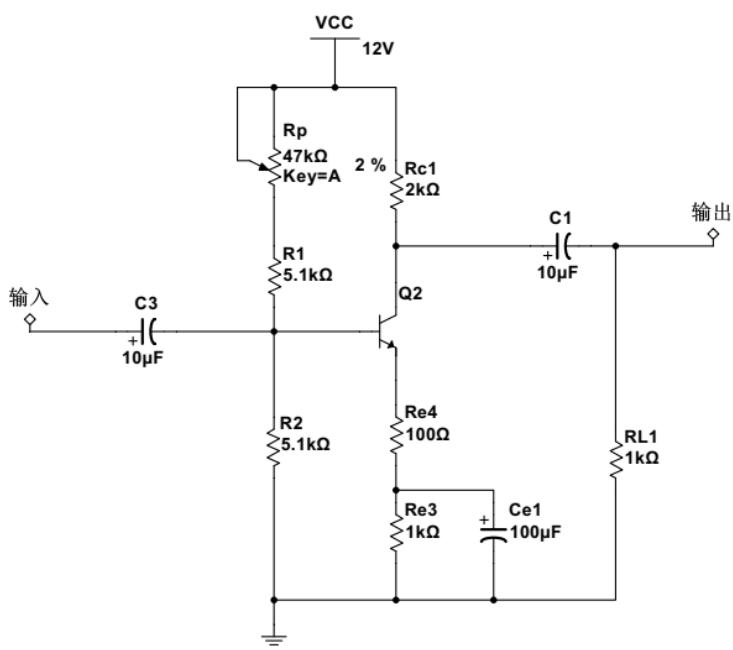
\includegraphics[width=0.6\textwidth]{1_Co_shot/circuit_exp1.png}
    \caption{共射放大电路原理图}
    \label{fig:circuit}
\end{figure}

\begin{table}[htbp]
    \centering
    \caption{电路元器件清单}
    \label{tab:components}
    \begin{tabular}{lll}
        \toprule
        \textbf{元件符号} & \textbf{参数值} & \textbf{作用} \\
        \midrule
        Q2 & 2N3904 & NPN型三极管，核心放大元件 \\
        Rp & \SI{47}{\kilo\ohm} & 可变电阻，用于精细调节静态工作点 \\
        R1, R2 & \SI{5.1}{\kilo\ohm} & 基极分压偏置电阻 \\
        Rc1 & \SI{2}{\kilo\ohm} & 集电极负载电阻 \\
        Re3, Re4 & \SI{1}{\kilo\ohm}, \SI{100}{\ohm} & 发射极电阻，稳定静态工作点 \\
        RL1 & \SI{1}{\kilo\ohm} & 交流负载电阻 \\
        C1, C3 & \SI{10}{\micro\farad} & 耦合电容，隔直通交 \\
        Ce1 & \SI{100}{\micro\farad} & 旁路电容，提高交流放大倍数 \\
        \bottomrule
    \end{tabular}
\end{table}

\paragraph{备注：}
\begin{itemize}
    \item 在实际测试中，滑动变阻器 Rp 接入电路的有效阻值为 \SI{3.7}{\kilo\ohm}。
    \item 在进行第二部分实验（测量输入输出电阻及幅频特性）时，为便于测量，在输入耦合电容 C3 前串联了一个 \SI{1}{\kilo\ohm} 的电阻 Rs。
\end{itemize}

% =================================================
% 第二部分：分析与计算
% =================================================
\section{分析与计算}
\label{sec:analysis}

本章节旨在通过理论计算，分析电路的静态工作点与交流动态参数，为实验测量提供理论依据。

\subsection{静态工作点(Q点)估算}

静态工作点的设置是为了保证三极管工作在放大区，避免信号失真。我们首先计算基极、集电极的静态电流以及集电极与发射极之间的静态电压。

\paragraph{计算前提与假设：}
\begin{itemize}
    \item 晶体管 Q2 (2N3904) 的电流放大系数 $\beta$ 设为典型值 150。
    \item 基极-发射极导通电压 $V_{BEQ} = \SI{0.7}{\volt}$。
    \item 电源电压 $V_{CC} = \SI{12}{\volt}$。
    \item 根据实验条件，滑动变阻器 Rp 的有效阻值为 $R_{p,eff} = \SI{3.7}{\kilo\ohm}$。
    \item 发射极总电阻 $R_E = R_{e3} + R_{e4} = \SI{1}{\kilo\ohm} + \SI{100}{\ohm} = \SI{1.1}{\kilo\ohm}$。
\end{itemize}

\paragraph{1. 基极等效电路计算：}
利用戴维南定理，计算基极偏置电路的等效电压 $V_{BB}$ 和等效电阻 $R_{BB}$。
\begin{align*}
    V_{BB} &= \frac{R_2}{R_p + R_1 + R_2} V_{CC} \\
           &= \frac{\SI{5.1}{\kilo\ohm}}{\SI{3.7}{\kilo\ohm} + \SI{5.1}{\kilo\ohm} + \SI{5.1}{\kilo\ohm}} \times \SI{12}{\volt} \approx \SI{4.40}{\volt} \\
    R_{BB} &= (R_p + R_1) \parallel R_2 \\
           &= (\SI{3.7}{\kilo\ohm} + \SI{5.1}{\kilo\ohm}) \parallel \SI{5.1}{\kilo\ohm} = \SI{8.8}{\kilo\ohm} \parallel \SI{5.1}{\kilo\ohm} \approx \SI{3.23}{\kilo\ohm}
\end{align*}

\paragraph{2. 静态电流与电压计算：}
根据基极-发射极回路的KVL方程，计算基极静态电流 $I_{BQ}$。
\begin{align*}
    I_{BQ} &= \frac{V_{BB} - V_{BEQ}}{R_{BB} + (1+\beta)R_E} \\
           &= \frac{\SI{4.40}{\volt} - \SI{0.7}{\volt}}{\SI{3.23}{\kilo\ohm} + (1+150) \times \SI{1.1}{\kilo\ohm}} \approx \SI{21.8}{\micro\ampere}
\end{align*}
由此可得集电极静态电流 $I_{CQ}$ 和发射极静态电流 $I_{EQ}$：
\begin{align*}
    I_{CQ} &= \beta I_{BQ} = 150 \times \SI{21.8}{\micro\ampere} \approx \SI{3.27}{\milli\ampere} \\
    I_{EQ} &= (1+\beta) I_{BQ} \approx I_{CQ} = \SI{3.27}{\milli\ampere}
\end{align*}
最后，根据集电极-发射极回路的KVL方程，计算管压降 $V_{CEQ}$。
\begin{align*}
    V_{CEQ} &= V_{CC} - I_{CQ}R_{c1} - I_{EQ}R_E \\
            &\approx V_{CC} - I_{CQ}(R_{c1} + R_E) \\
            &= \SI{12}{\volt} - \SI{3.27}{\milli\ampere} \times (\SI{2}{\kilo\ohm} + \SI{1.1}{\kilo\ohm}) \approx \SI{1.86}{\volt}
\end{align*}
由于 $V_{CEQ} \approx \SI{1.86}{\volt} > V_{CE,sat} (\approx \SI{0.2}{\volt})$，因此晶体管工作在放大区，静态工作点设置合理。

\subsection{交流动态特性分析}

基于静态工作点，我们可以建立交流小信号模型，估算电路的电压放大倍数 $A_u$、输入电阻 $R_i$ 和输出电阻 $R_o$。

\paragraph{1. 晶体管交流参数：}
首先计算晶体管的发射结动态电阻 $r_{be}$。
\begin{align*}
    r_e &= \frac{V_T}{I_{EQ}} \approx \frac{\SI{26}{\milli\volt}}{\SI{3.27}{\milli\ampere}} \approx \SI{7.95}{\ohm} \\
    r_{be} &= (1+\beta)r_e = (1+150) \times \SI{7.95}{\ohm} \approx \SI{1.20}{\kilo\ohm}
\end{align*}

\paragraph{2. 电压放大倍数 $A_u$：}
在交流通路中，电容 $C_{e1}$ 旁路了电阻 $R_{e3}$，因此交流发射极电阻为 $R_{e4}$。交流负载为 $R_{c1}$ 和 $R_{L1}$ 的并联。
\begin{align*}
    R'_L &= R_{c1} \parallel R_{L1} = \SI{2}{\kilo\ohm} \parallel \SI{1}{\kilo\ohm} = \frac{2 \times 1}{2+1}\,\si{\kilo\ohm} \approx \SI{667}{\ohm} \\
    A_u &= -\frac{\beta R'_L}{r_{be} + (1+\beta)R_{e4}} \\
        &= -\frac{150 \times \SI{667}{\ohm}}{\SI{1.20}{\kilo\ohm} + (1+150) \times \SI{100}{\ohm}} \approx -5.81
\end{align*}
理论计算的电压放大倍数约为 -5.81，负号表示输出信号与输入信号反相。

\paragraph{3. 输入电阻 $R_i$：}
放大电路的输入电阻是基极偏置等效电阻 $R_{BB}$ 与晶体管输入电阻 $R_{ib}$ 的并联。
\begin{align*}
    R_{ib} &= r_{be} + (1+\beta)R_{e4} = \SI{1.20}{\kilo\ohm} + (1+150) \times \SI{100}{\ohm} = \SI{16.3}{\kilo\ohm} \\
    R_i &= R_{BB} \parallel R_{ib} = \SI{3.23}{\kilo\ohm} \parallel \SI{16.3}{\kilo\ohm} \approx \SI{2.70}{\kilo\ohm}
\end{align*}

\paragraph{4. 输出电阻 $R_o$：}
放大电路的输出电阻约等于集电极电阻 $R_{c1}$。
\begin{equation*}
    R_o \approx R_{c1} = \SI{2}{\kilo\ohm}
\end{equation*}

% =================================================
% 第三部分：测试方案与测试结果
% =================================================
\section{测试方案与测试结果}
\label{sec:results}

本章节将详细描述实验的测试流程，展示并分析测量数据，最后将实验结果与理论值进行对比。以下是实际电路连接的照片，如图 \ref{fig:actual_circuit} 所示。

\begin{figure}[H] 
    \centering
    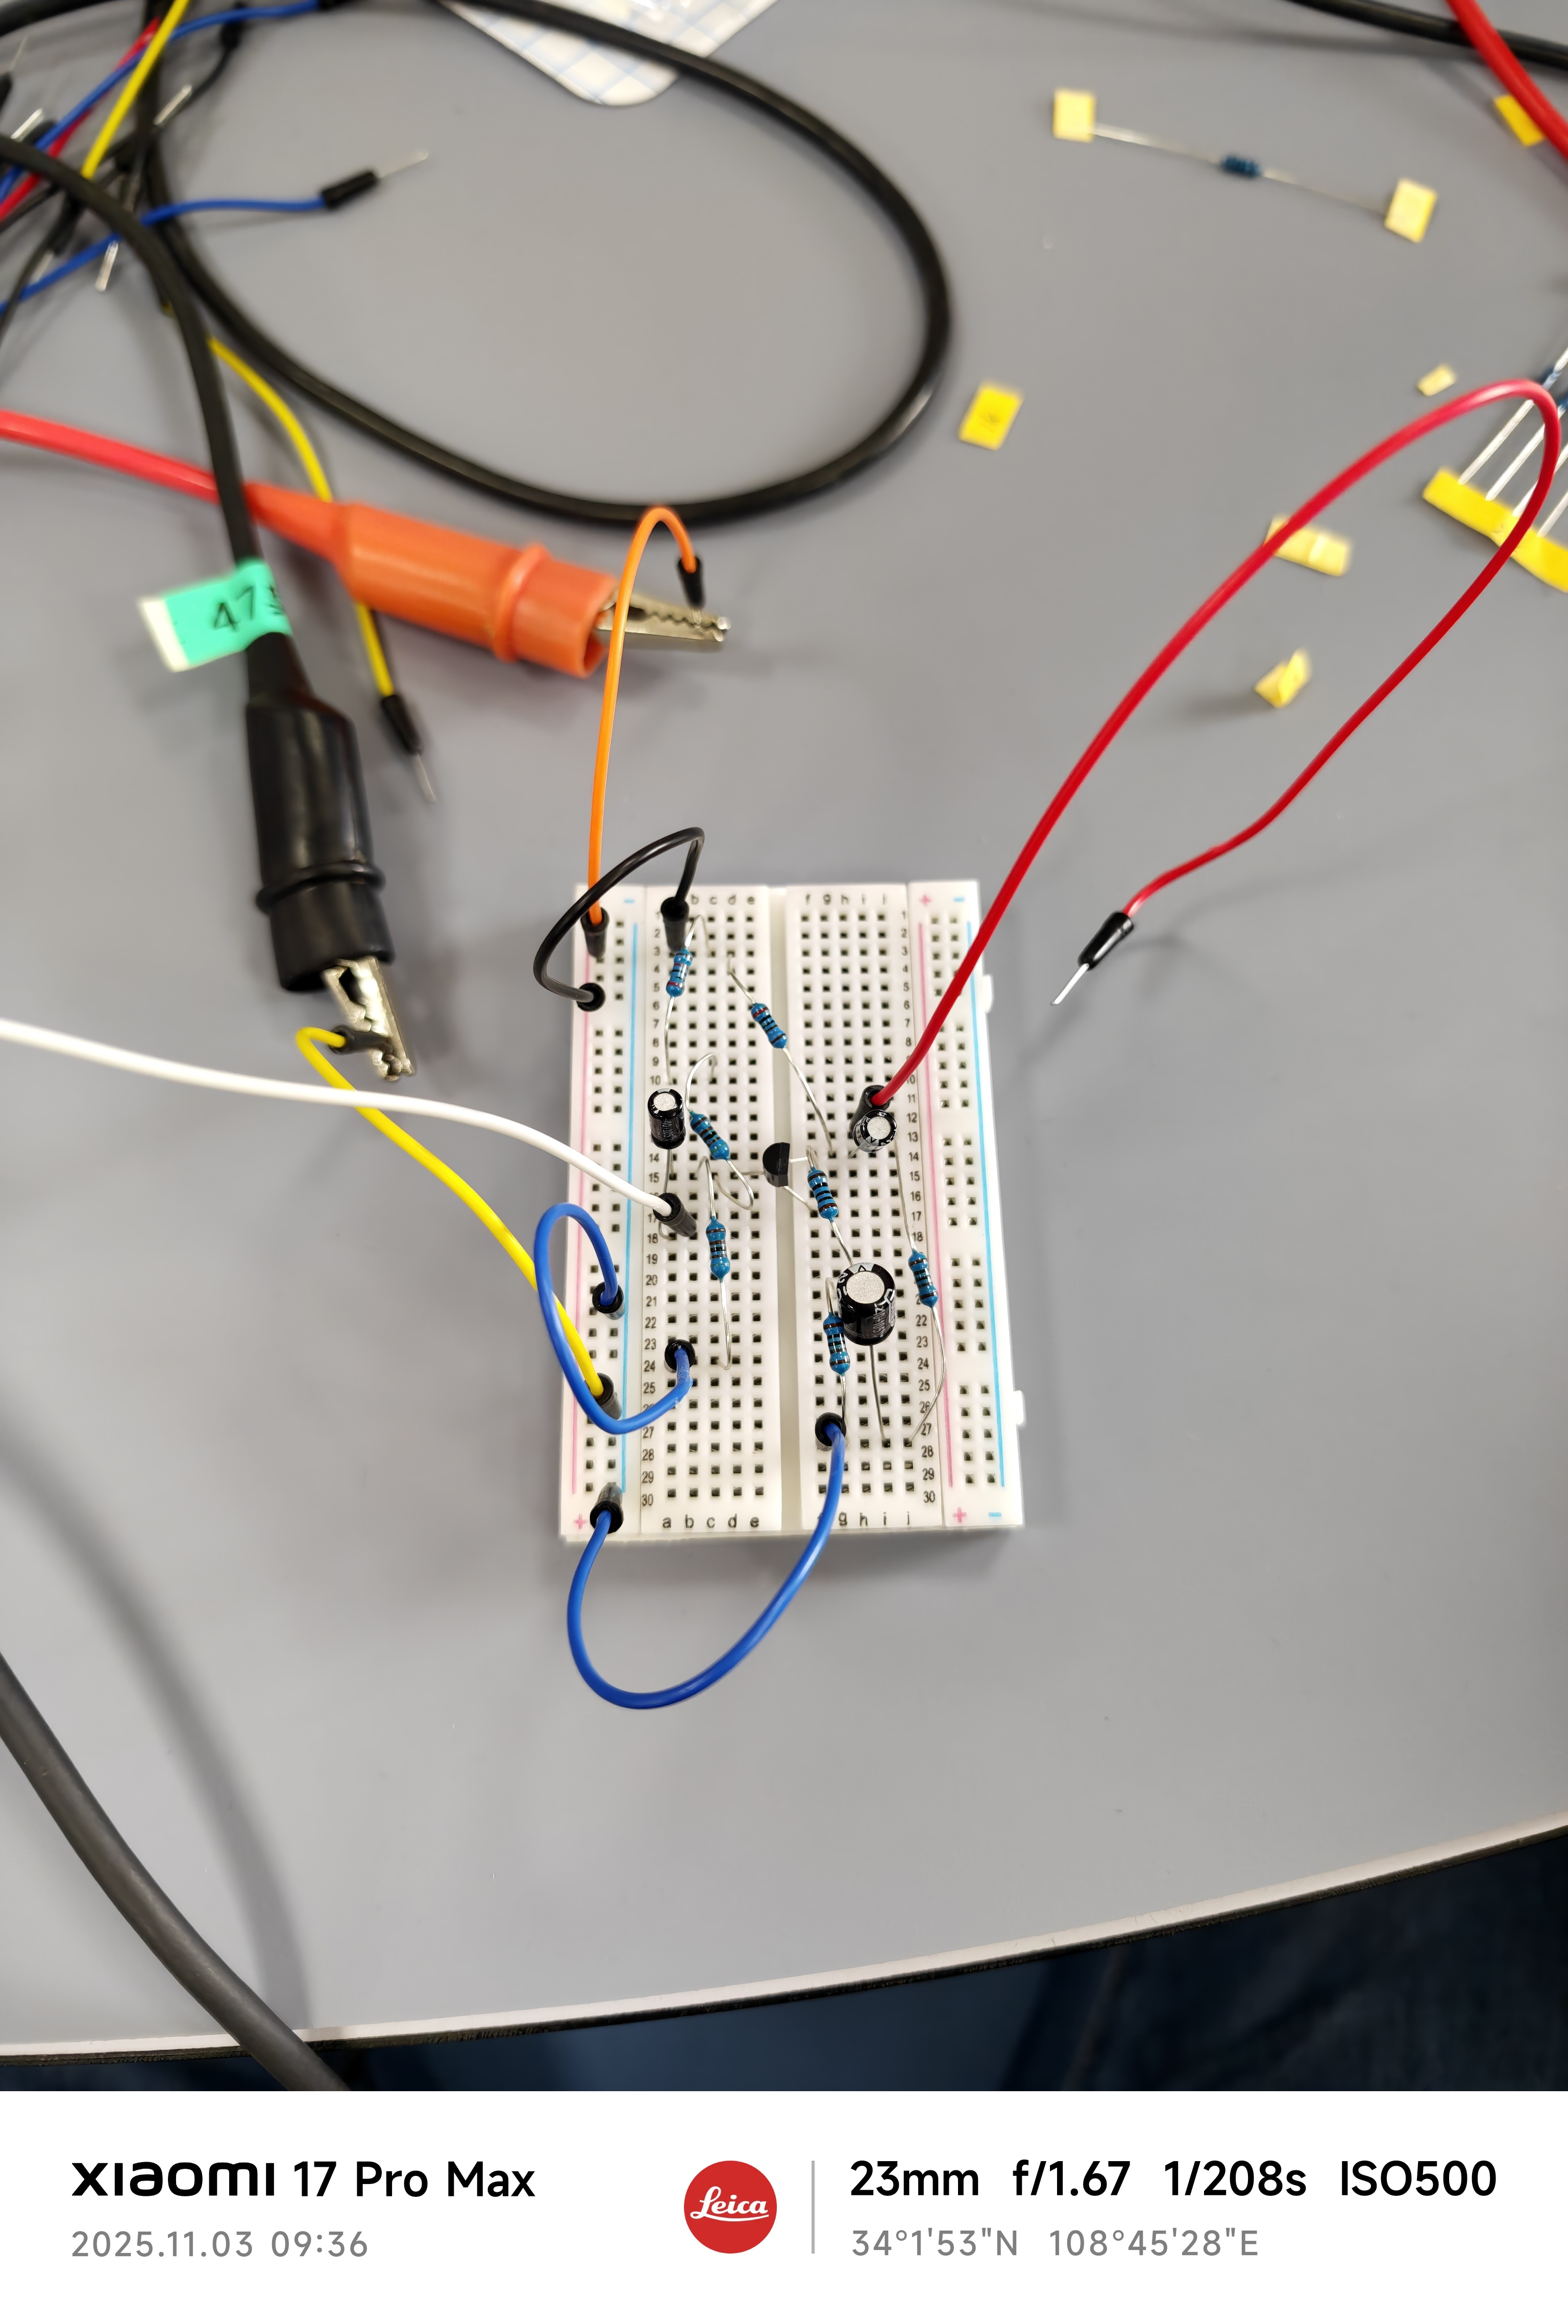
\includegraphics[width=0.3\textwidth]{1_Co_shot/actual_circuit.jpg}
    \caption{实际电路连接照片}
    \label{fig:actual_circuit}
\end{figure}

\subsection{第一部分：静态工作点与电压放大倍数}

\paragraph{1. 测试方案：}
使用直流电源提供 $\pm\SI{12}{\volt}$ 的工作电压。信号发生器产生一个频率为 \SI{1}{\kilo\hertz} 的正弦波作为输入信号 $v_i$。通过调节信号发生器的幅度和可变电阻 Rp，在示波器上观察输出信号 $v_o$，直至其上下削波（饱和失真与截止失真）的幅度基本对称，此时电路的静态工作点达到最优。该状态下的波形如图 \ref{fig:q_point} 所示。

\begin{figure}[H] % 使用 [H] 强制图片在此处显示
    \centering
    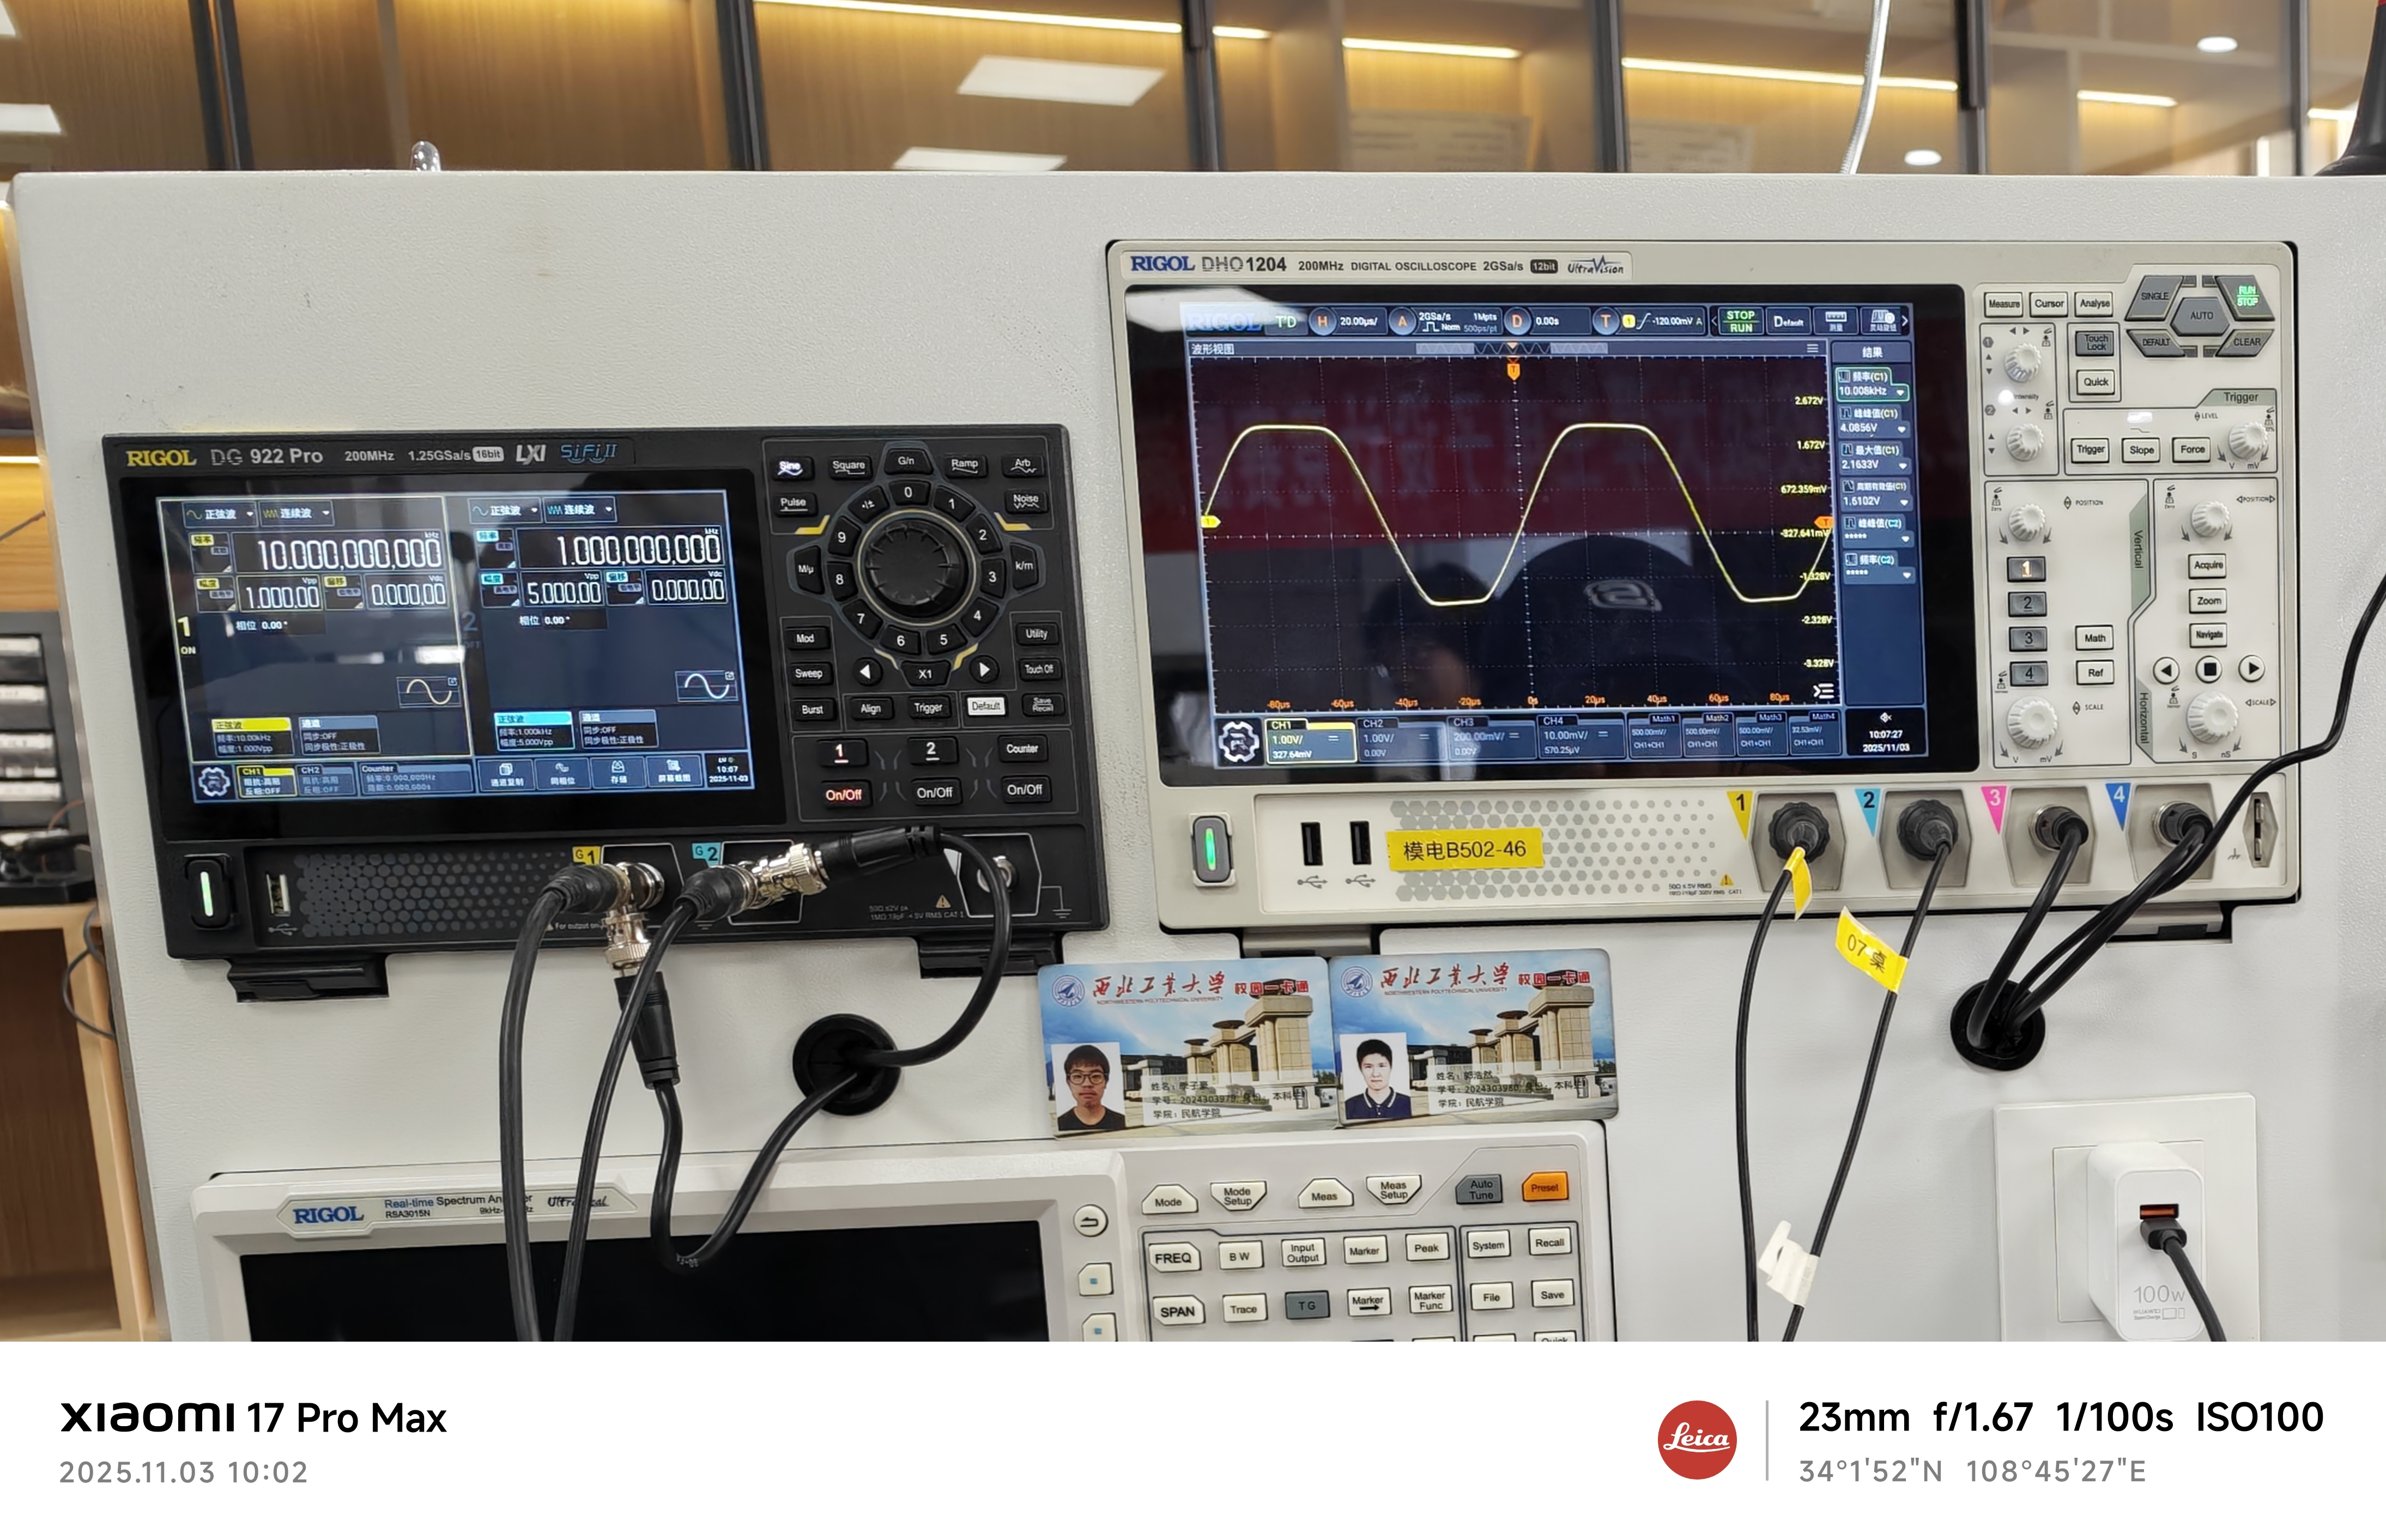
\includegraphics[width=0.6\textwidth]{1_Co_shot/scope_q_point.jpg}
    \caption{输出波形达到最大不失真动态范围（最佳Q点）}
    \label{fig:q_point}
\end{figure}

\paragraph{2. 电压放大倍数测量：}
在最佳工作点下，使用万用表的交流电压档（有效值）测量输入电压 $V_i$ 和输出电压 $V_o$，测量读数如图 \ref{fig:volt_gain_measure} 所示。
\begin{itemize}
    \item 输入电压有效值 $V_i = \SI{34.388}{\milli\volt}$
    \item 输出电压有效值 $V_o = \SI{207.219}{\milli\volt}$
\end{itemize}

\begin{figure}[htbp]
    \centering
    \begin{subfigure}[b]{0.48\textwidth}
        \centering
        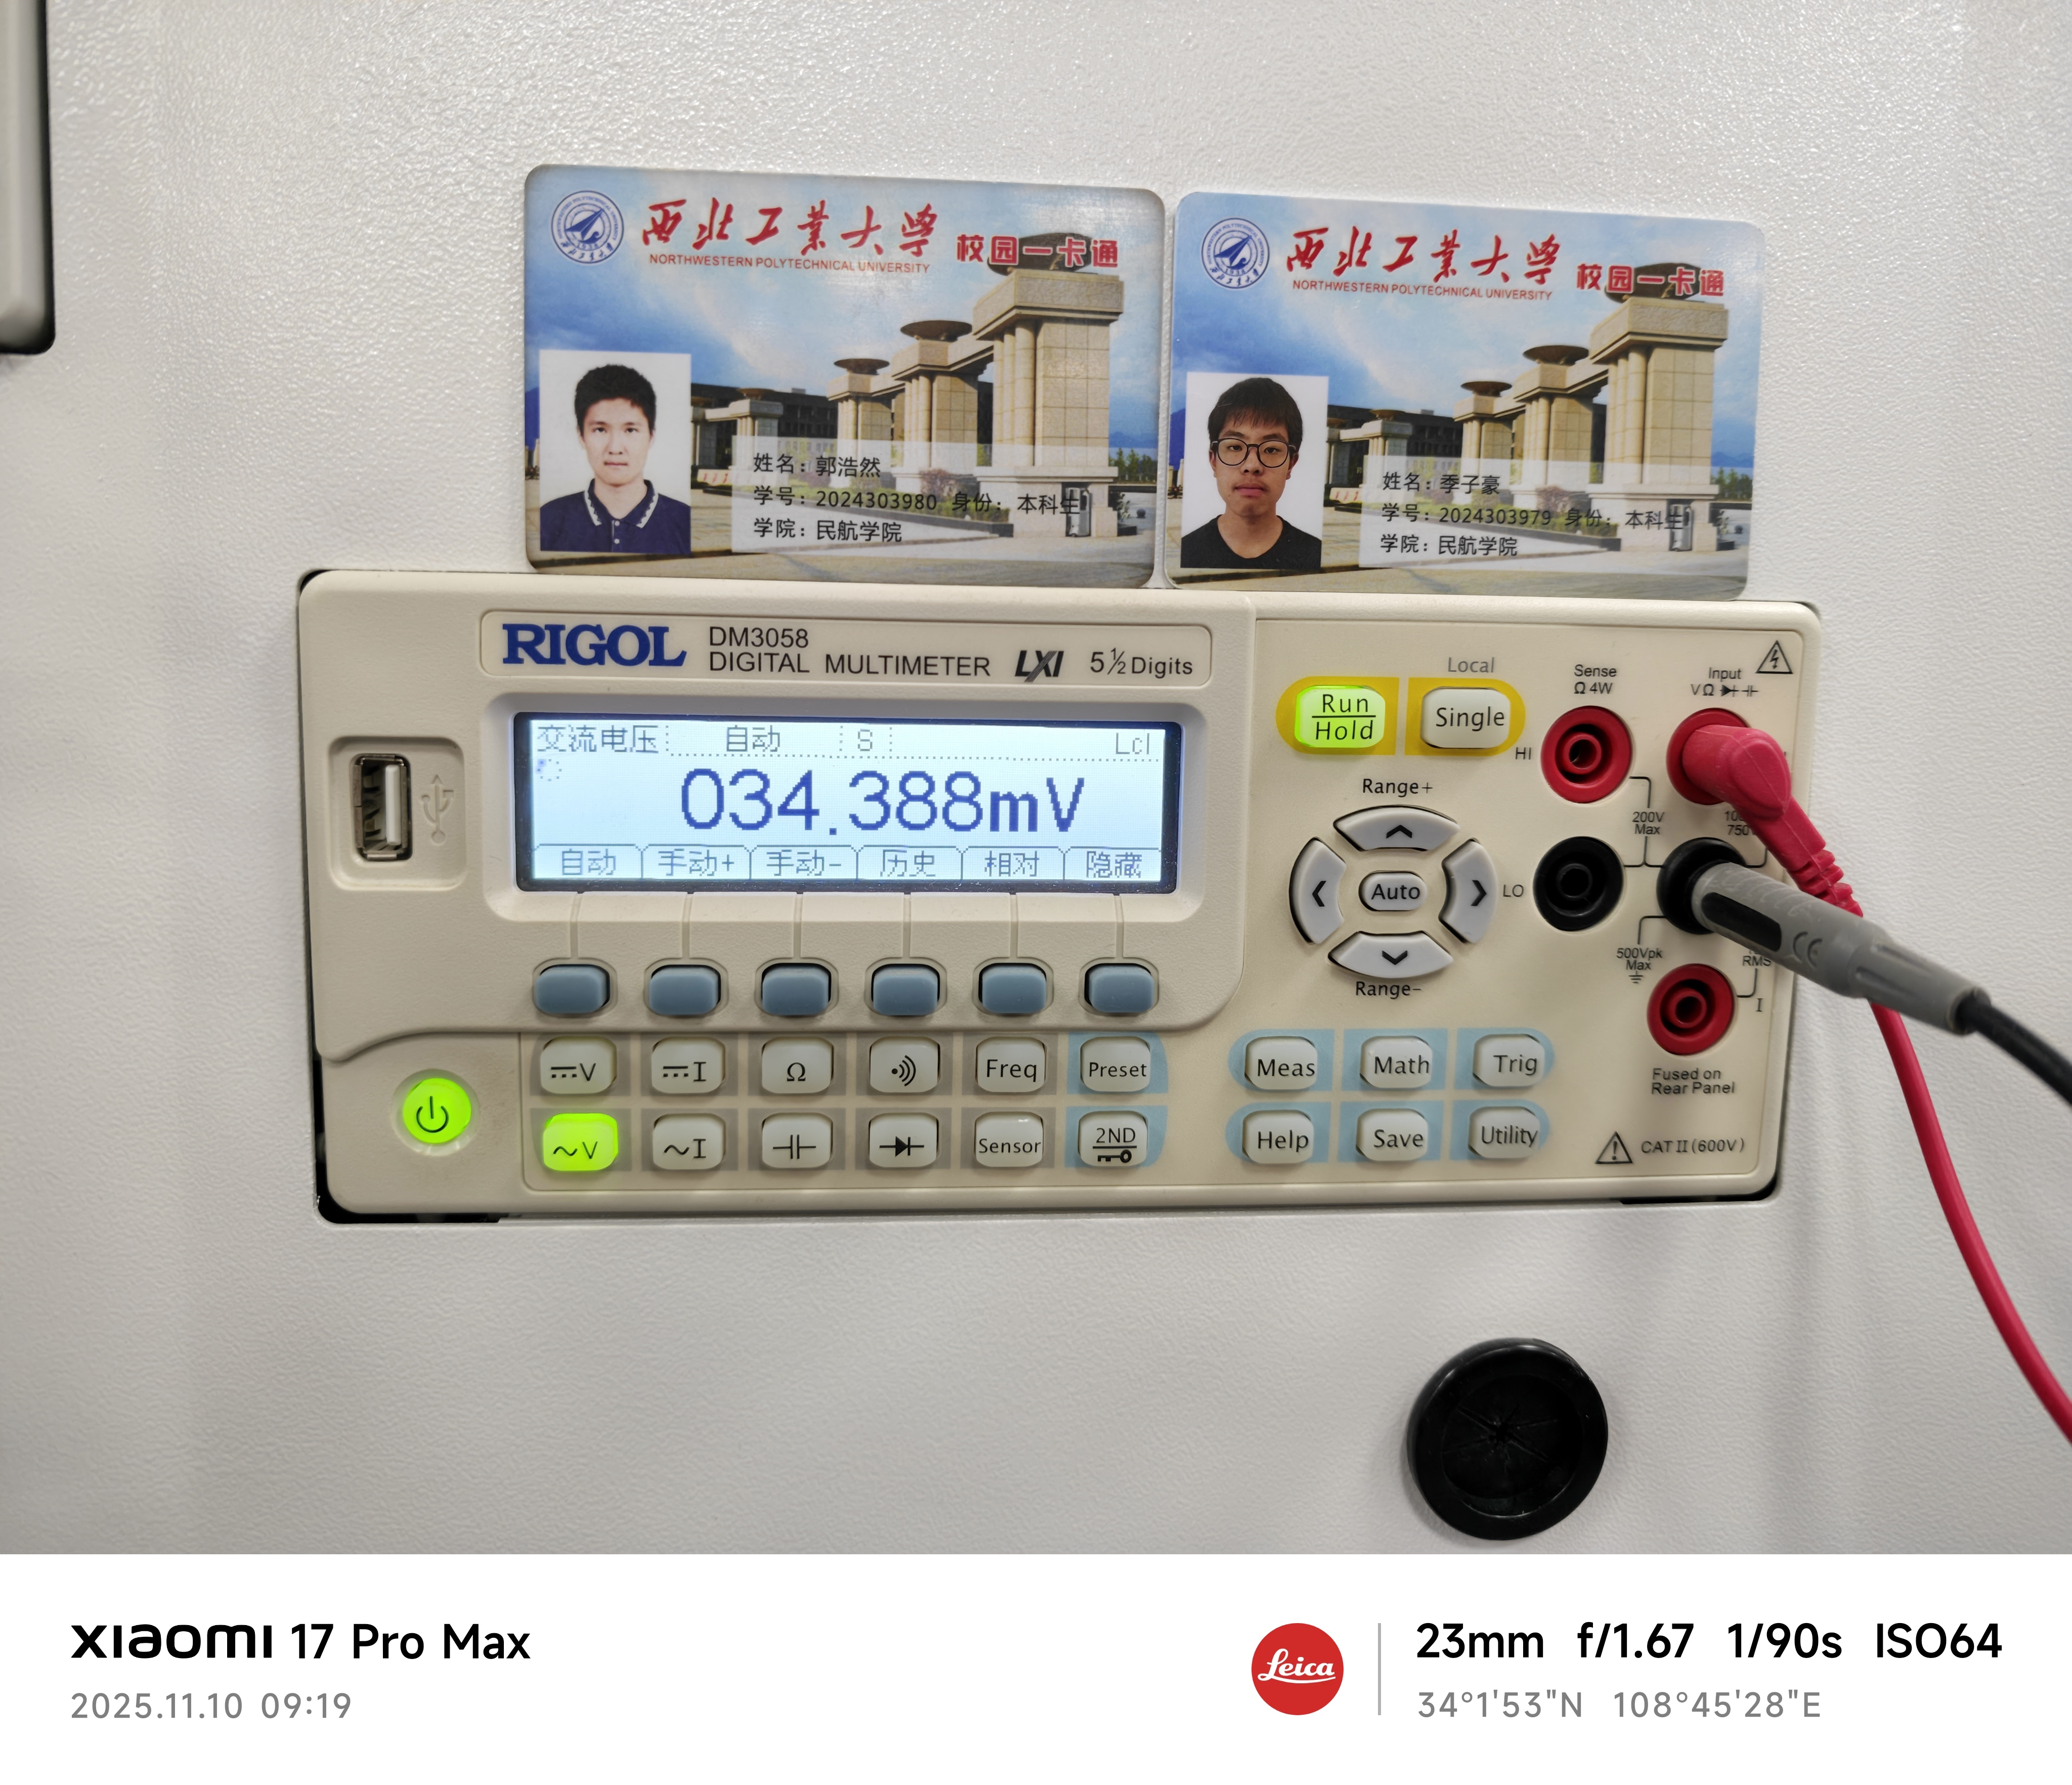
\includegraphics[width=\textwidth]{1_Co_shot/av2.jpg}
        \caption{输入电压 $V_i$ 测量}
        \label{fig:vi_gain}
    \end{subfigure}
    \hfill % 水平填充
    \begin{subfigure}[b]{0.48\textwidth}
        \centering
        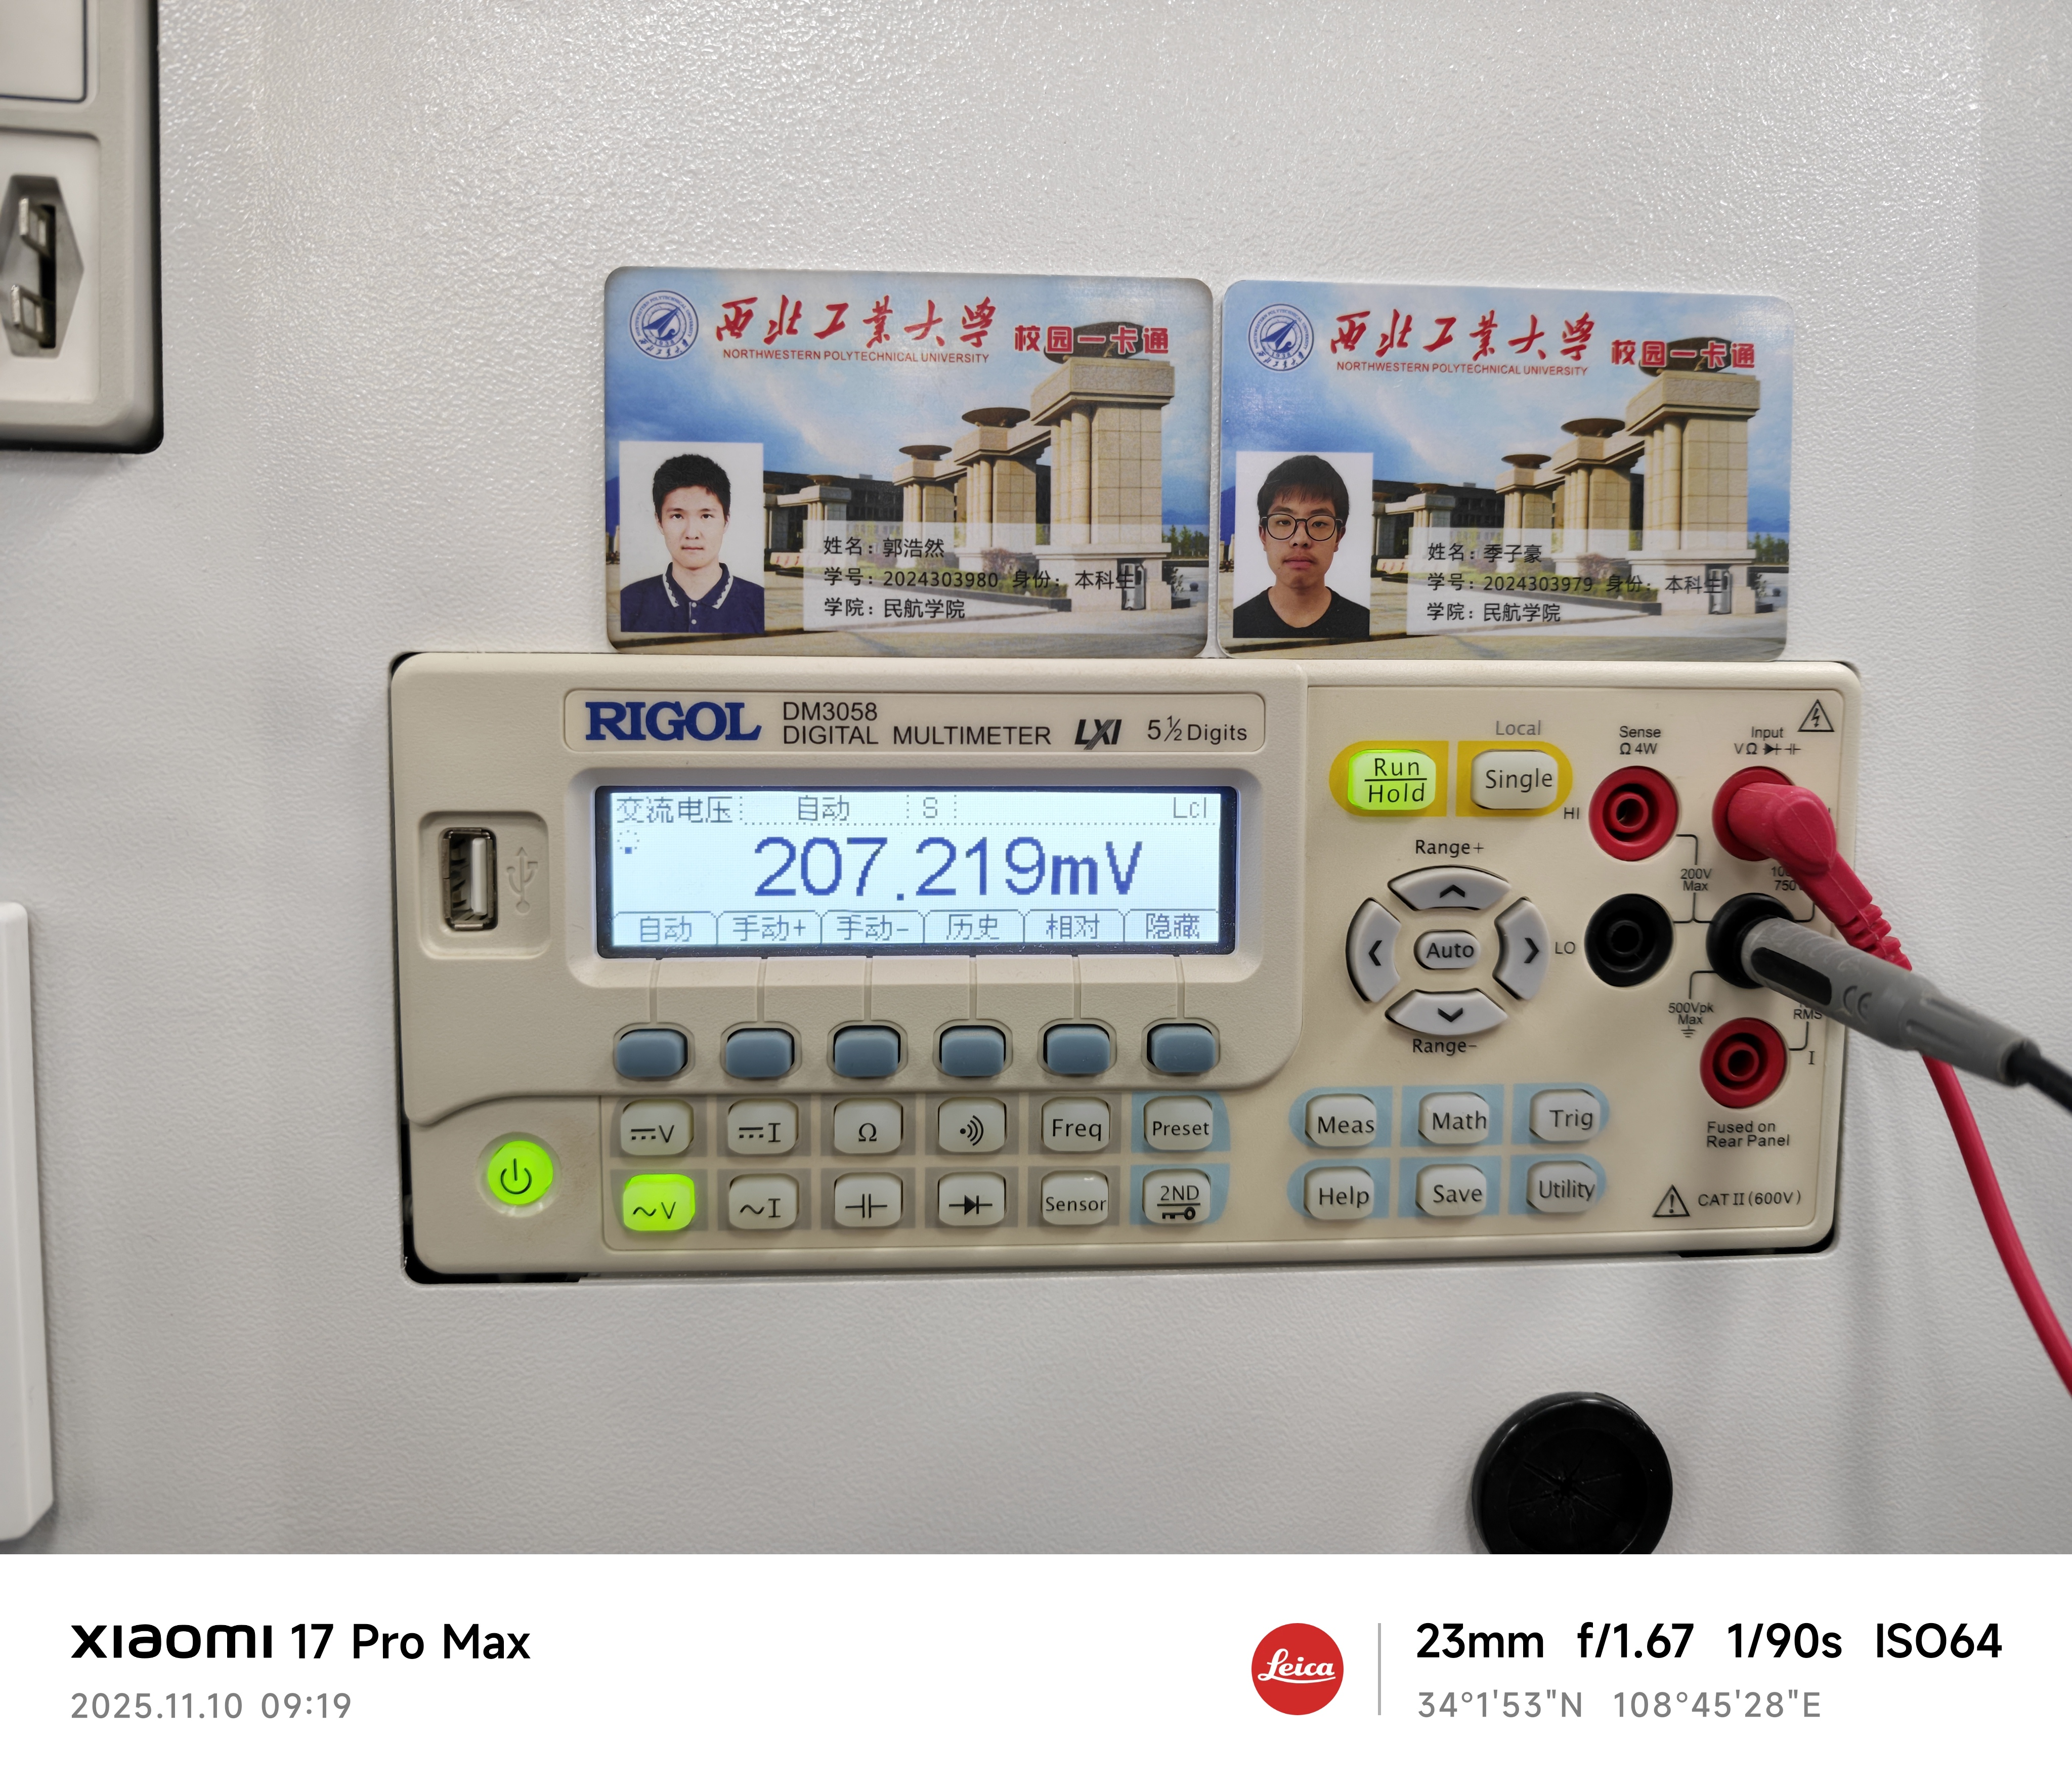
\includegraphics[width=\textwidth]{1_Co_shot/av1.jpg}
        \caption{输出电压 $V_o$ 测量}
        \label{fig:vo_gain}
    \end{subfigure}
    \caption{电压放大倍数测量读数}
    \label{fig:volt_gain_measure}
\end{figure}

电压放大倍数 $A_u$ 的计算如下：
\begin{equation}
    A_u = \frac{V_o}{V_i} = \frac{\SI{207.219}{\milli\volt}}{\SI{34.388}{\milli\volt}} \approx 6.03
\end{equation}
实验测得的电压放大倍数约为 6.03。其理论计算值为 -5.81，两者绝对值大小接近，差异可能源于晶体管 $\beta$ 值的实际偏差。

\paragraph{3. 静态基极电压测量与分析：}
分别测量在有交流信号输入时（示波器直流耦合读数）和输入端接地时（万用表直流电压档读数）的基极直流电压。
\begin{itemize}
    \item 有信号输入时基极直流偏置 $V_1 = \SI{4.2234}{\volt}$
    \item 输入信号接地时基极直流电压 $V_2 = \SI{4.2068}{\volt}$
\end{itemize}
\textbf{分析：} 理论上，一个设计良好的偏置电路，其静态工作点不应受到小信号交流输入的影响。实验测得 $V_1$ 和 $V_2$ 的值非常接近，相对误差仅为 $0.4\%$，这证明了本电路静态工作点的稳定性。

\subsection{第二部分：输入/输出电阻与幅频特性}

\paragraph{测试说明：}
为便于测量输入电阻，本部分实验在输入耦合电容 C3 前串联了一个 $R_s = \SI{1}{\kilo\ohm}$ 的已知电阻，但包括输出电阻在内的其他元件并未改动（未按照PPT上的仿真电路修改）。
\paragraph{1. 输入电阻 $R_i$ 测量：}
根据测试方法，测量信号源电压 $V_s$ 和放大电路输入端电压 $V_i$。
\begin{itemize}
    \item 信号源电压 $V_s = \SI{33.898}{\milli\volt}$
    \item 电路输入端电压 $V_i = \SI{32.021}{\milli\volt}$
\end{itemize}
输入电流 $I_i$ 为流过串联电阻 $R_s = \SI{1}{\kilo\ohm}$ 的电流，即 $I_i = (V_s - V_i) / R_s$。因此输入电阻 $R_i$ 计算如下：
\begin{equation}
    R_i = \frac{V_i}{I_i} = \frac{V_i}{(V_s - V_i) / R_s} = \frac{\SI{32.021}{\milli\volt}}{(\SI{33.898}{\milli\volt} - \SI{32.021}{\milli\volt})} \times \SI{1}{\kilo\ohm} \approx \SI{17.06}{\kilo\ohm}
\end{equation}
实验测得输入电阻约为 \SI{17.06}{\kilo\ohm}。该值与理论计算值 \SI{2.70}{\kilo\ohm} 存在较大差异，这主要是因为理论计算中采用的晶体管 $\beta$ 值 (150) 可能远小于实际值。输入电阻对 $\beta$ 值非常敏感，较高的 $\beta$ 值会显著增大晶体管的动态电阻 $r_{be}$，从而导致整体输入电阻 $R_i$ 增大。

\paragraph{2. 输出电阻 $R_o$ 测量：}
测量空载时的输出电压 $V_o$ 和接入负载 $R_{L} = \SI{2}{\kilo\ohm}$ 时的输出电压 $V_L$。
\begin{itemize}
    \item 空载输出电压 $V_o = \SI{207.219}{\milli\volt}$
    \item 带载输出电压 $V_L = \SI{116.47}{\milli\volt}$
\end{itemize}
根据电压分压原理，输出电阻 $R_o$ 计算如下：
根据电压分压原理，输出电阻 $R_o$ 计算如下：
\begin{equation}
    R_o = \left( \frac{V_o}{V_L} - 1 \right) \times R_{L1} = \left( \frac{\SI{207.219}{\milli\volt}}{\SI{116.472}{\milli\volt}} - 1 \right) \times \SI{2}{\kilo\ohm} \approx \SI{1.567}{\kilo\ohm}
\end{equation}
实验测得输出电阻约为 \SI{1.567}{\kilo\ohm}，该测量结果与理论估算值 $R_o \approx R_{c1} = \SI{2}{\kilo\ohm}$ 基本吻合，验证了理论分析的准确性。

\begin{figure}[H]
    \centering
    \begin{subfigure}[b]{0.48\textwidth}
        \centering
        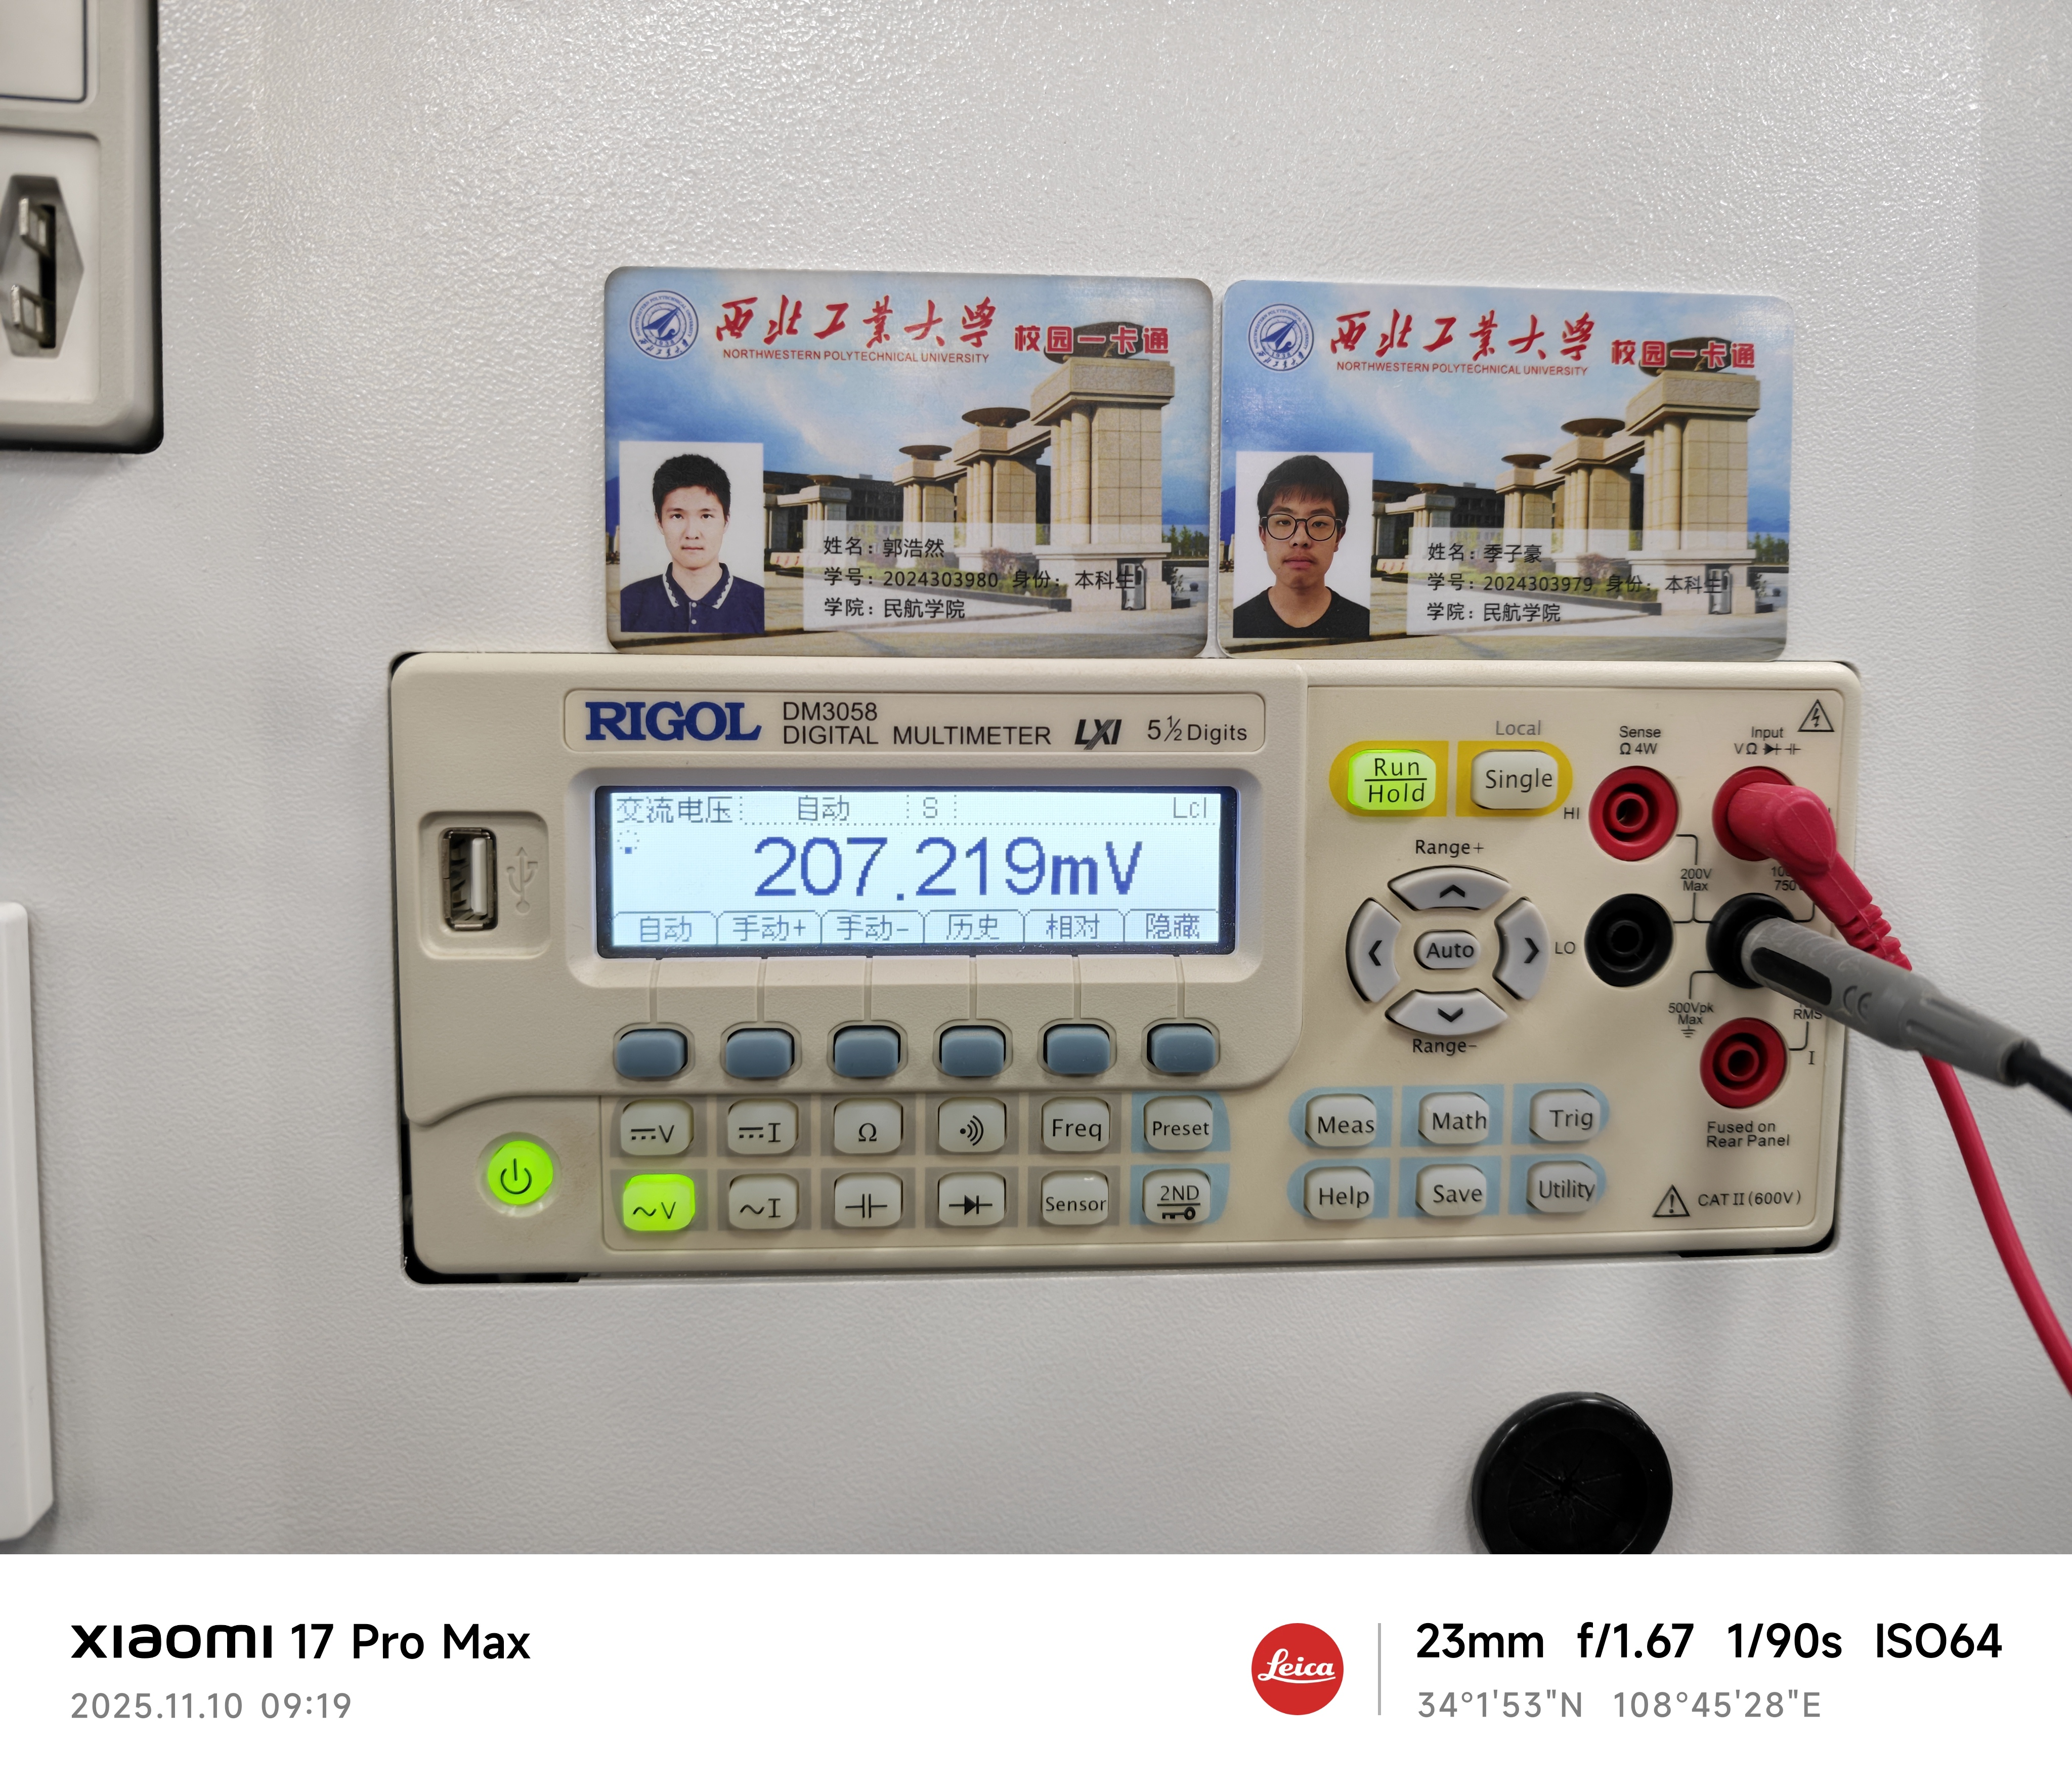
\includegraphics[width=\textwidth]{1_Co_shot/av1.jpg}
        \caption{空载输出电压 $V_o$ 测量}
        \label{fig:vo_noload}
    \end{subfigure}
    \hfill
    \begin{subfigure}[b]{0.48\textwidth}
        \centering
        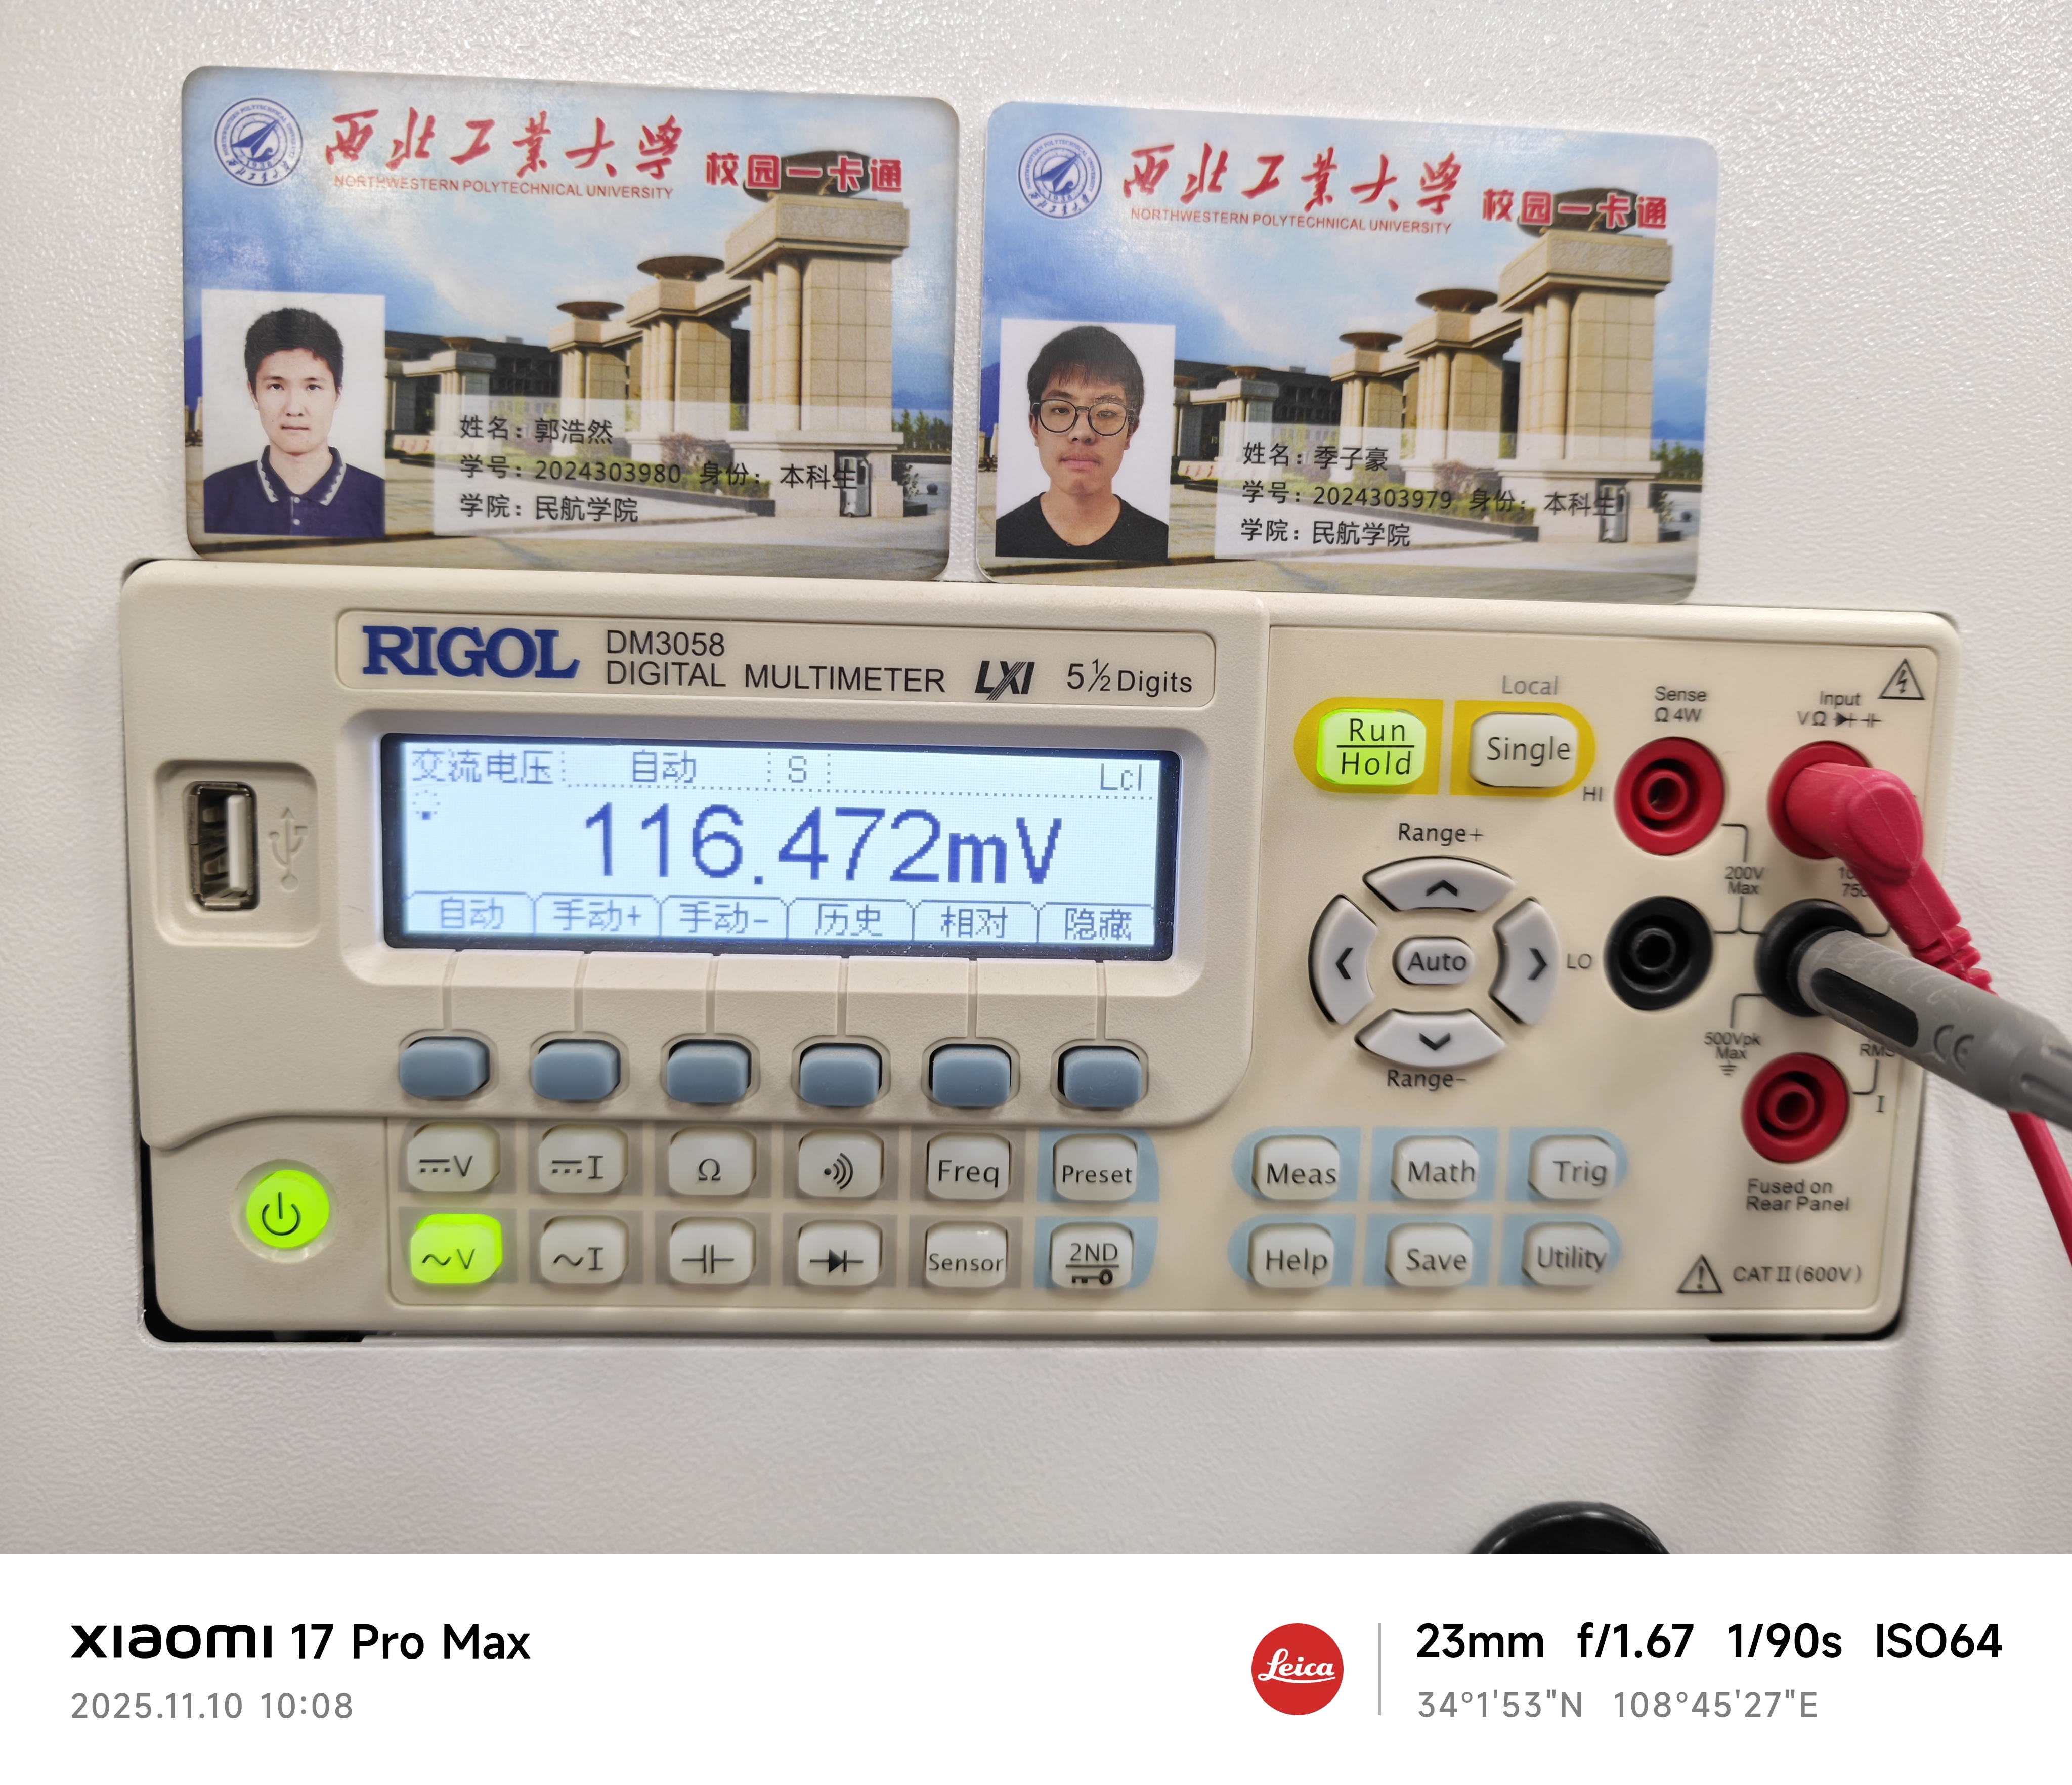
\includegraphics[width=\textwidth]{1_Co_shot/vl.jpg}
        \caption{带载输出电压 $V_L$ 测量}
        \label{fig:vl_load}
    \end{subfigure}
    \caption{输出电阻测量读数}
    \label{fig:res_out_measure}
\end{figure}

\paragraph{3. 幅频特性与带宽：}
在 \SI{1}{\kilo\hertz} 中频段，测得输出电压峰峰值为 $V_{opp,mid} = \SI{466.58}{\milli\volt}$。根据 $-3\text{dB}$ 定义，截止频率点对应的输出电压峰峰值为 $V_{opp, -3dB} \approx \SI{329.9}{\milli\volt}$。通过扫频测量，找到截止频率点，其示波器截图如图 \ref{fig:freq_response1} 所示。
\begin{itemize}
    \item \textbf{低频截止频率 $f_L$：} 在 $f = \SI{25}{\hertz}$ 时，测得 $V_{opp} = \SI{332.54}{\milli\volt}$。
    \item \textbf{高频截止频率 $f_H$：} 在 $f = \SI{1.8}{\mega\hertz}$ 时，测得 $V_{opp} = \SI{324.53}{\milli\volt}$。
\end{itemize}

\begin{figure}[H]
    \centering
    \begin{subfigure}[b]{0.48\textwidth}
        \centering
        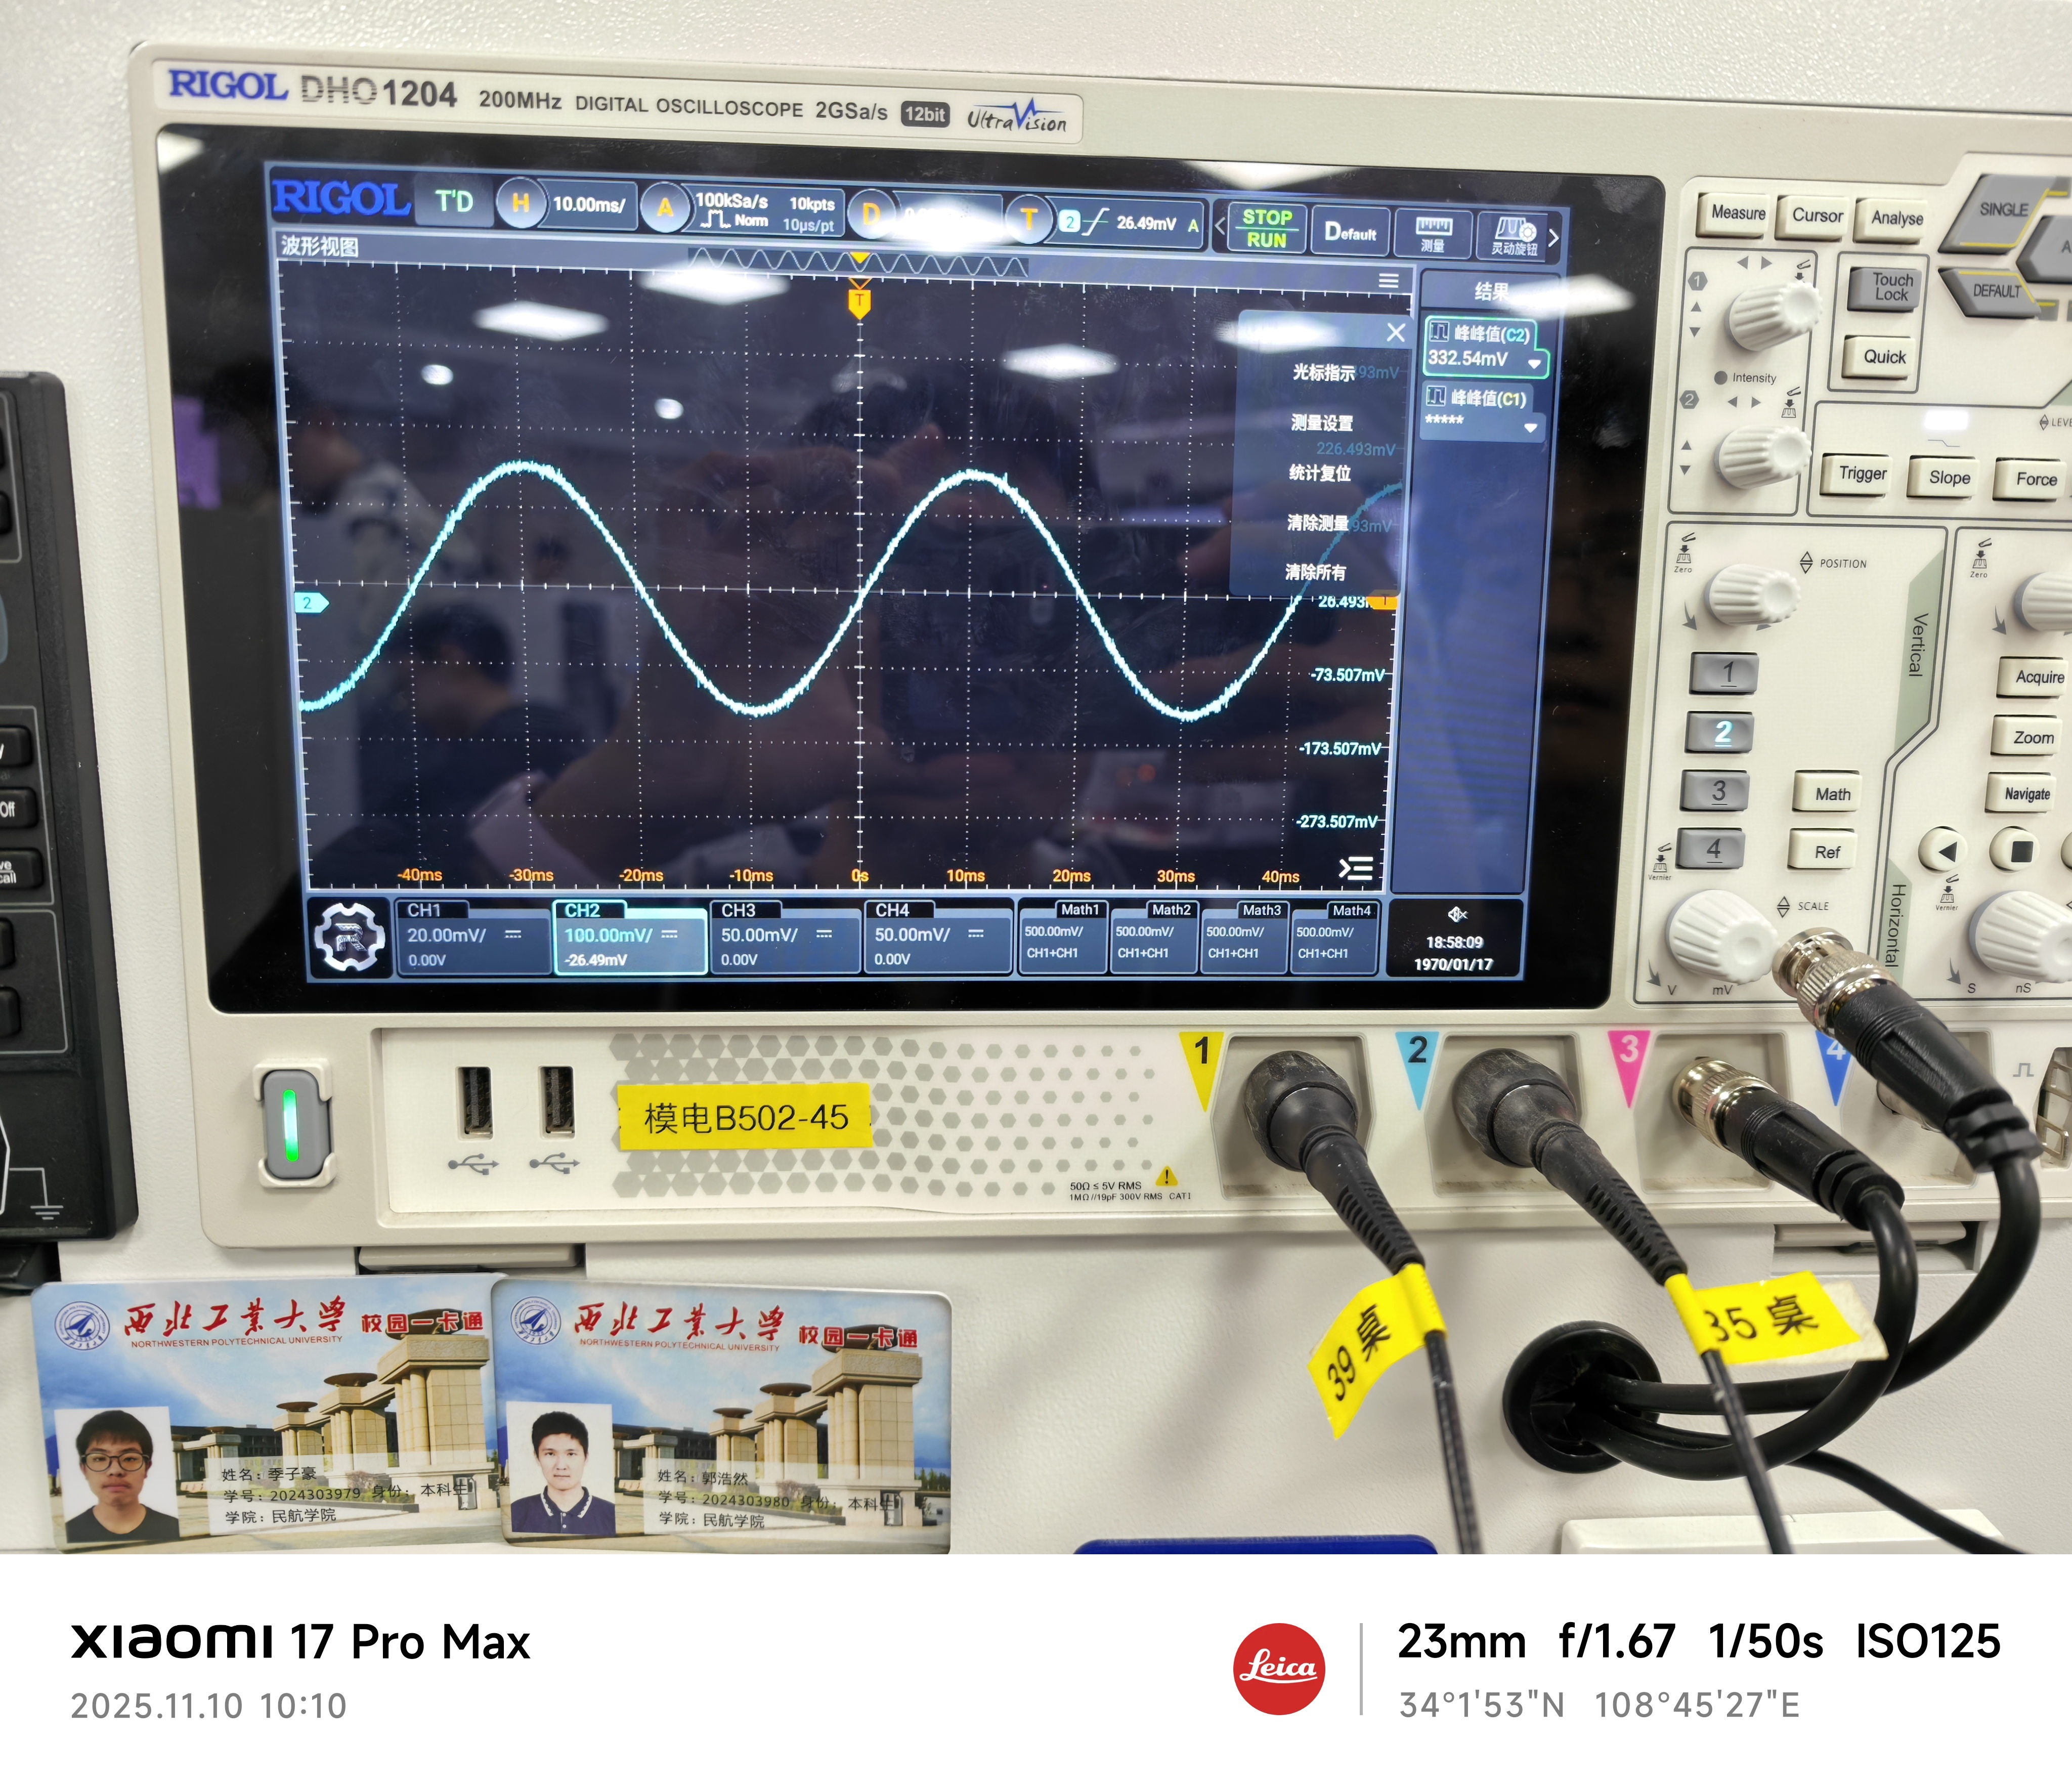
\includegraphics[width=\textwidth]{1_Co_shot/25hz.jpg}
        \caption{低频截止频率 $f_L$ 处波形}
        \label{fig:low_cutoff}
    \end{subfigure}
    \hfill
    \begin{subfigure}[b]{0.48\textwidth}
        \centering
        \includegraphics[width=\textwidth]{1_Co_shot/1.8mhz.jpg}
        \caption{高频截止频率 $f_H$ 处波形}
        \label{fig:high_cutoff}
    \end{subfigure}
    \caption{上下截止频率测量}
    \label{fig:freq_response1}
\end{figure}

因此，该放大电路的通频带宽度 BW 为：
\begin{equation}
    \text{BW} = f_H - f_L = \SI{1.8}{\mega\hertz} - \SI{25}{\hertz} \approx \SI{1.8}{\mega\hertz}
\end{equation}

拟合得到的幅频特性曲线如图 \ref{fig:bode_plot} 所示。
\begin{figure}[H]
    \centering
    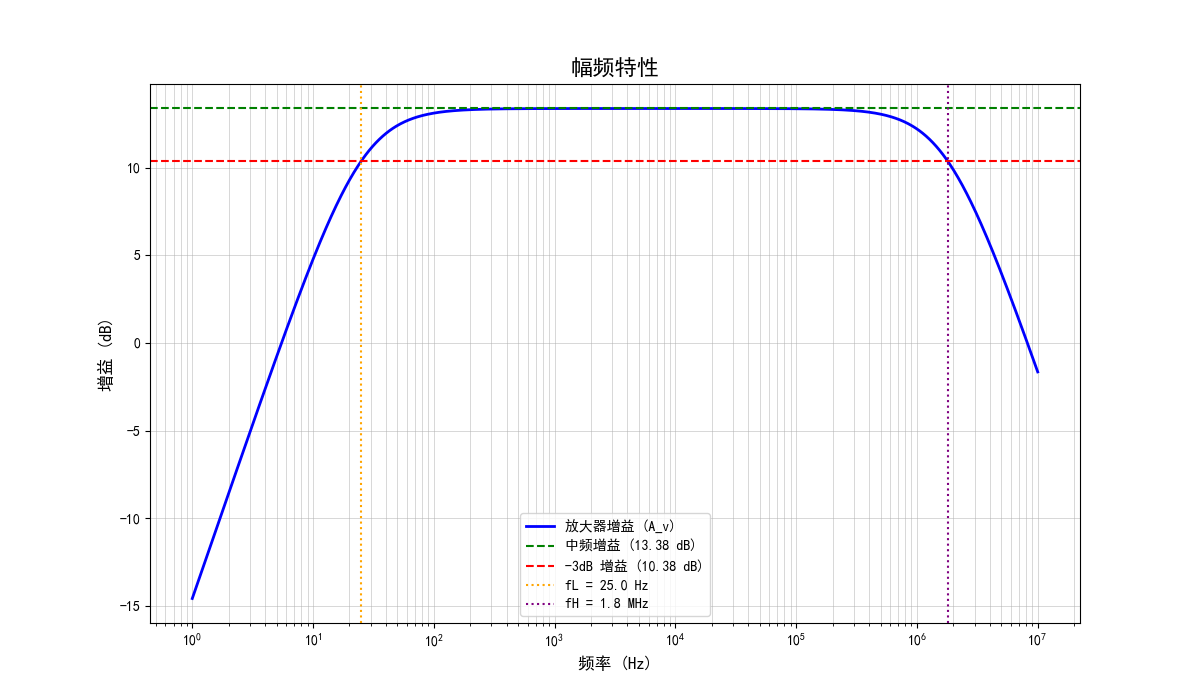
\includegraphics[width=0.9\textwidth]{1_Co_shot/A_jw.png}
    \caption{幅频特性曲线拟合}
    \label{fig:bode_plot}
\end{figure}

% =================================================
% 第二章：运算放大器类型与主要指标  
% =================================================
\clearpage
\chapter{运算放大器类型与主要指标}\label{chap:opamp_metrics}

\section{实验目的}\label{sec:opamp_purpose}
\begin{enumerate}
    \item 查阅并对比 LM324 与 OP07 两种运算放大器的芯片规格书 (datasheet)。
    \item 搭建电压缓冲器电路，测量并比较两种芯片的输入失调电压 ($V_{\text{OS}}$) 与共模输入范围。
    \item 测试 LM324 构成的电压缓冲器电路的幅频特性，并计算其通频带。
\end{enumerate}

% ===================================================================
% 章节：实验器件介绍与参数对比
% (采用 minipage 实现图表并排)
% ===================================================================
\section{实验器件介绍与参数对比}\label{sec:opamp_chips}

\subsection{LM324 低功耗四路运算放大器}
LM324 是一款内部集成了四个独立的、高增益、内部频率补偿运算放大器的集成电路。它专为单电源或双电源操作而设计，在宽电压范围内具有低功耗的特点，非常适合用于各类通用模拟电路。

\begin{figure}[H]
    \centering
    \begin{minipage}[c]{0.45\textwidth}
        \centering
        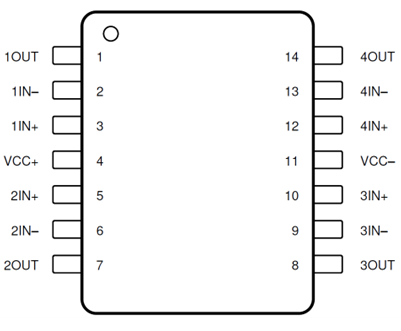
\includegraphics[width=\linewidth]{2_Op_amp/lm324_pinout.png} % <-- 请替换为您的LM324引脚图路径
    \end{minipage}
    \hfill % 在两个 minipage 之间提供弹性空间
    \begin{minipage}[c]{0.5\textwidth}
        \centering
        \captionof{table}{LM324 芯片引脚功能定义} % 使用 captionof 将表格标题放入 figure 环境
        \label{tab:lm324_pins}
        \small % 缩小表格字体以适应布局
        \begin{tabular}{ccl}
            \toprule
            \textbf{引脚} & \textbf{名称} & \textbf{功能定义} \\
            \midrule
            1  & 1OUT & 运放1输出端 \\
            2  & 1IN- & 运放1反相输入端 \\
            3  & 1IN+ & 运放1同相输入端 \\
            4  & VCC+ & 正电源 \\
            5  & 2IN+ & 运放2同相输入端 \\
            6  & 2IN- & 运放2反相输入端 \\
            7  & 2OUT & 运放2输出端 \\
            8  & 3OUT & 运放3输出端 \\
            9  & 3IN- & 运放3反相输入端 \\
            10 & 3IN+ & 运放3同相输入端 \\
            11 & VCC- & 负电源或接地 \\
            12 & 4IN+ & 运放4同相输入端 \\
            13 & 4IN- & 运放4反相输入端 \\
            14 & 4OUT & 运放4输出端 \\
            \bottomrule
        \end{tabular}
    \end{minipage}
    \caption{LM324 芯片引脚图及功能表}
    \label{fig:lm324_layout}
\end{figure}

\subsection{OP07 高精度运算放大器}
OP07 是一款具有极低输入失调电压的高精度单运算放大器。它通过内部的失调电压调整电路实现了优异的直流性能，非常适合用于精密仪器、传感器信号放大等要求苛刻的应用场景。

\begin{figure}[H]
    \centering
    \begin{minipage}[c]{0.45\textwidth}
        \centering
        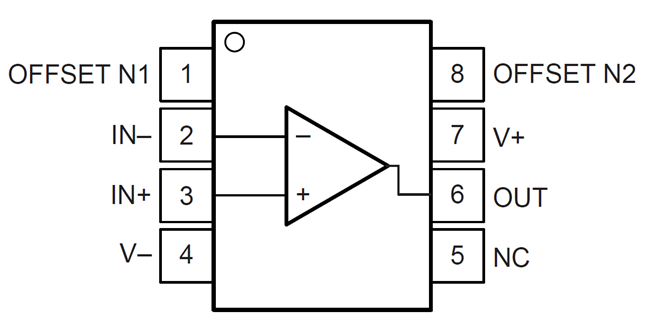
\includegraphics[width=\linewidth]{2_Op_amp/op07_pinout.png}
    \end{minipage}
    \hfill
    \begin{minipage}[c]{0.5\textwidth}
        \centering
        \captionof{table}{OP07 芯片引脚功能定义}
        \label{tab:op07_pins}
        \begin{tabular}{ccl}
            \toprule
            \textbf{引脚} & \textbf{名称} & \textbf{功能定义} \\
            \midrule
            1 & OFFSET N1 & 失调电压调整 \\
            2 & IN-       & 反相输入端 \\
            3 & IN+       & 同相输入端 \\
            4 & V-        & 负电源 \\
            5 & NC        & 未连接 \\
            6 & OUT       & 输出端 \\
            7 & V+        & 正电源 \\
            8 & OFFSET N2 & 失调电压调整 \\
            \bottomrule
        \end{tabular}
    \end{minipage}
    \caption{OP07 芯片引脚图及功能表}
    \label{fig:op07_layout}
\end{figure}

\subsection{主要技术指标对比}
根据两种芯片的规格书，其关键性能指标对比如表 \ref{tab:opamp_specs} 所示。

\begin{table}[H]
    \centering
    \caption{LM324 与 OP07 主要指标对比 (典型值)}
    \label{tab:opamp_specs}
    \begin{tabular}{lll}
        \toprule
        \textbf{参数} & \textbf{LM324} & \textbf{OP07} \\
        \midrule
        电源电压范围 & 单电源 \SI{3}{\volt} \textasciitilde{} \SI{32}{\volt} & 双电源 $\pm$\SI{3}{\volt} \textasciitilde{} $\pm$\SI{18}{\volt} \\
                     & 或双电源 $\pm$\SI{1.5}{\volt} \textasciitilde{} $\pm$\SI{16}{\volt} & \\
        输入失调电压 & \SI{2}{\milli\volt} & \SI{30}{\micro\volt} \\
        开环增益 & \SI{100}{\volt/\milli\volt} & \SI{300}{\volt/\milli\volt} \\
        压摆率 & \SI{0.5}{\volt/\micro\second} & \SI{0.3}{\volt/\micro\second} \\
        共模输入范围 & \SI{0}{\volt} \textasciitilde{} $V_{CC} - \SI{1.5}{\volt}$ & $\pm$\SI{13.5}{\volt} (于 $\pm$\SI{15}{\volt} 电源) \\
        \bottomrule
    \end{tabular}
\end{table}


\section{实验原理}\label{sec:opamp_principle}

\subsection{核心电路与概念}
\subsubsection{1. 电压缓冲器}
电压缓冲器 (Voltage Buffer)，也称电压跟随器 (Voltage Follower)，是一种输出电压精确跟随输入电压的电路，其电压增益约等于 1。它具有高输入阻抗、低输出阻抗的特点，常用于电路的隔离、阻抗匹配等场合。其电路如图 \ref{fig:buffer_circuit} 所示，通过将输出端直接反馈到反相输入端实现。

\begin{figure}[H] % 使用 [H] 选项，强制图片出现在此处
    \centering
    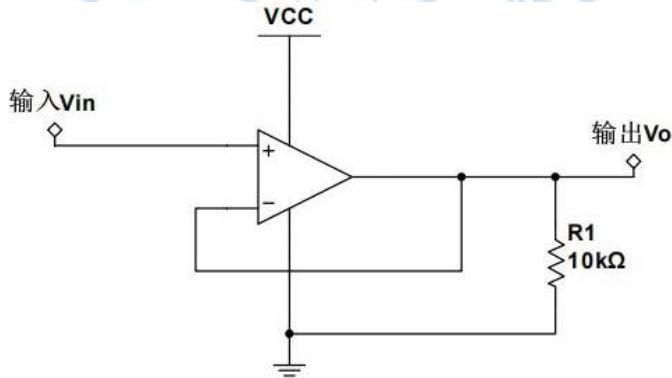
\includegraphics[width=0.5\textwidth]{2_Op_amp/buffer_circuit.png} % <-- 请替换为您的电压缓冲器电路图路径
    \caption{电压缓冲器电路原理图}
    \label{fig:buffer_circuit}
\end{figure}


\subsubsection{2. 输入失调电压 ($V_{\text{OS}}$)}
理想运算放大器在两输入端电压相等时，输出应为零。而实际运放由于内部差分对管的不完全对称，在输入差模电压为零时，输出仍有一个微小的非零直流电压。为使输出归零，需在输入端施加一个补偿性的差模电压，该电压即为输入失调电压 $V_{\text{OS}}$。

\subsubsection{3. 共模输入范围 (Common-Mode Input Range)}
共模输入范围是指运放能够保持正常线性工作的、施加在两个输入端上的公共电压范围。当输入信号的共模电压超出此范围时，运放的增益、线性度等性能会急剧下降，甚至进入饱和区，无法正常工作。对于单电源供电的 LM324，其共模输入范围通常为 \SI{0}{\volt} 到 $V_{CC} - \SI{1.5}{\volt}$。

\section{实验内容与步骤}\label{sec:opamp_content}
\subsection{实验内容}
\begin{enumerate}
    \item 测量并记录由 LM324 与 OP07 芯片构成的电压缓冲器的输入失调电压。
    \item 搭建电压缓冲器电路，测试并确定 LM324 芯片在 \SI{12}{\volt} 单电源供电下的共模输入范围。
    \item 测试 LM324 构成的电压缓冲器电路的幅频特性，确定其上限截止频率和通频带。
\end{enumerate}

\subsection{实验步骤}
\subsubsection{测量运放失调电压}
\begin{enumerate}
    \item 按照图 \ref{fig:simulation_circuit} 搭建电路，使用 LM324 芯片，采用 \SI{12}{\volt} 单电源供电。
    \item 将输入端 $V_{\text{in}}$ 接地 (\SI{0}{\volt})。
    \item 使用数字万用表的直流毫伏档，精确测量输出端电压 $V_{\text{out}}$。由于是电压跟随器，此时 $V_{\text{out}} \approx V_{\text{OS}}$。
    \item 更换芯片为 OP07，重复步骤 2-3，记录其输出电压。对比两者差异并与规格书核对。
\end{enumerate}

\subsubsection{测量共模输入范围}
\begin{enumerate}
    \item 使用 LM324 构成的电压缓冲器电路。
    \item 将输入电压 $V_{\text{in}}$ 从 \SI{0}{\volt} 开始，通过直流电源缓慢增加。
    \item 同时用两个万用表监测 $V_{\text{in}}$ 和 $V_{\text{out}}$ 的电压值。
    \item 记录当 $V_{\text{out}}$ 开始不再精确跟随 $V_{\text{in}}$ (例如，$V_{\text{out}}$ 停止上升) 时的临界输入电压 $V_{\text{in,max}}$。
    \item 该电路的共模输入范围即为 $[\SI{0}{\volt}, V_{\text{in,max}}]$。
\end{enumerate}

\subsubsection{测试幅频特性}
\begin{enumerate}
    \item 使用 LM324 构成的电压缓冲器电路。将输入信号源更换为函数信号发生器，输出正弦波。
    \item 设置输入信号的直流偏置为 \SI{6}{\volt}，峰峰值为 \SI{200}{\milli\volt}。
    \item 首先将频率设置在中频段 (如 \SI{1}{\kilo\hertz})，用示波器测量并记录此时的输出电压幅值 $A_m$。
    \item 保持输入信号幅值不变，逐渐降低频率。由于运放可放大直流信号，理论上下限截止频率 $f_L$ 为 \SI{0}{\hertz}。
    \item 逐渐升高频率，用示波器观察输出电压幅值。当幅值下降到 $0.707 \times A_m$ 时，记录此时的频率，即为上限截止频率 $f_H$。
    \item 计算通频带 $f_{BW} = f_H - f_L$。
\end{enumerate}

\section{实验电路方案}\label{sec:opamp_scheme}
本实验采用图 \ref{fig:simulation_circuit} 所示的电路方案。该电路为标准的电压跟随器配置，输出端接有 \SI{10}{\kilo\ohm} 的负载电阻 $R_L$。整个电路由 \SI{12}{\volt} 的单电源供电。

\begin{figure}[H] % 使用 [H] 选项，强制图片出现在此处
    \centering
    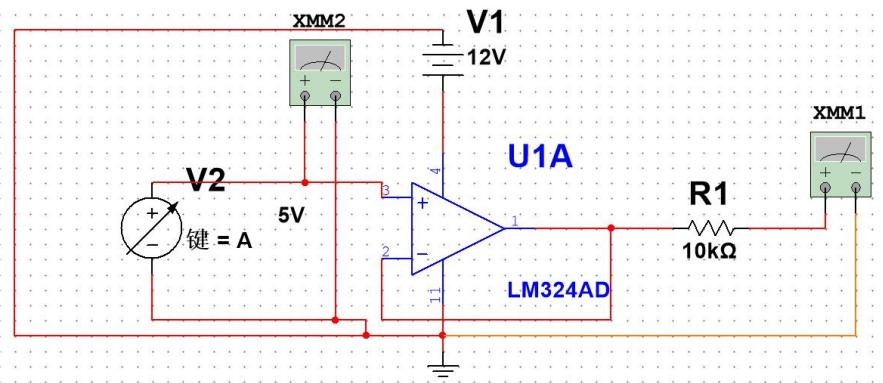
\includegraphics[width=0.6\textwidth]{2_Op_amp/simulation_circuit.jpg} % <-- 请替换为您的仿真电路图路径
    \caption{实验用电压缓冲器电路图 (LM324)}
    \label{fig:simulation_circuit}
\end{figure}


\section{测试与数据记录}\label{sec:opamp_data}
\subsection{测试用仪器}
\begin{itemize}
    \item 直流稳压电源
    \item 数字示波器
    \item 函数信号发生器
    \item 数字万用表
    \item 实验芯片：LM324, OP07
    \item \SI{10}{\kilo\ohm} 电阻
    \item 导线及面包板
\end{itemize}

\subsection{实验结果与数据记录}
\subsubsection{运放失调电压测量}
通过将电压跟随器的输入端接地，直接在输出端用数字万用表测量得到的电压即为输入失调电压 $V_{\text{OS}}$。两种芯片的实测情况如图 \ref{fig:vos_measurement} 所示。

\begin{figure}[H]
    \centering
    \begin{subfigure}[b]{0.48\textwidth}
        \centering
        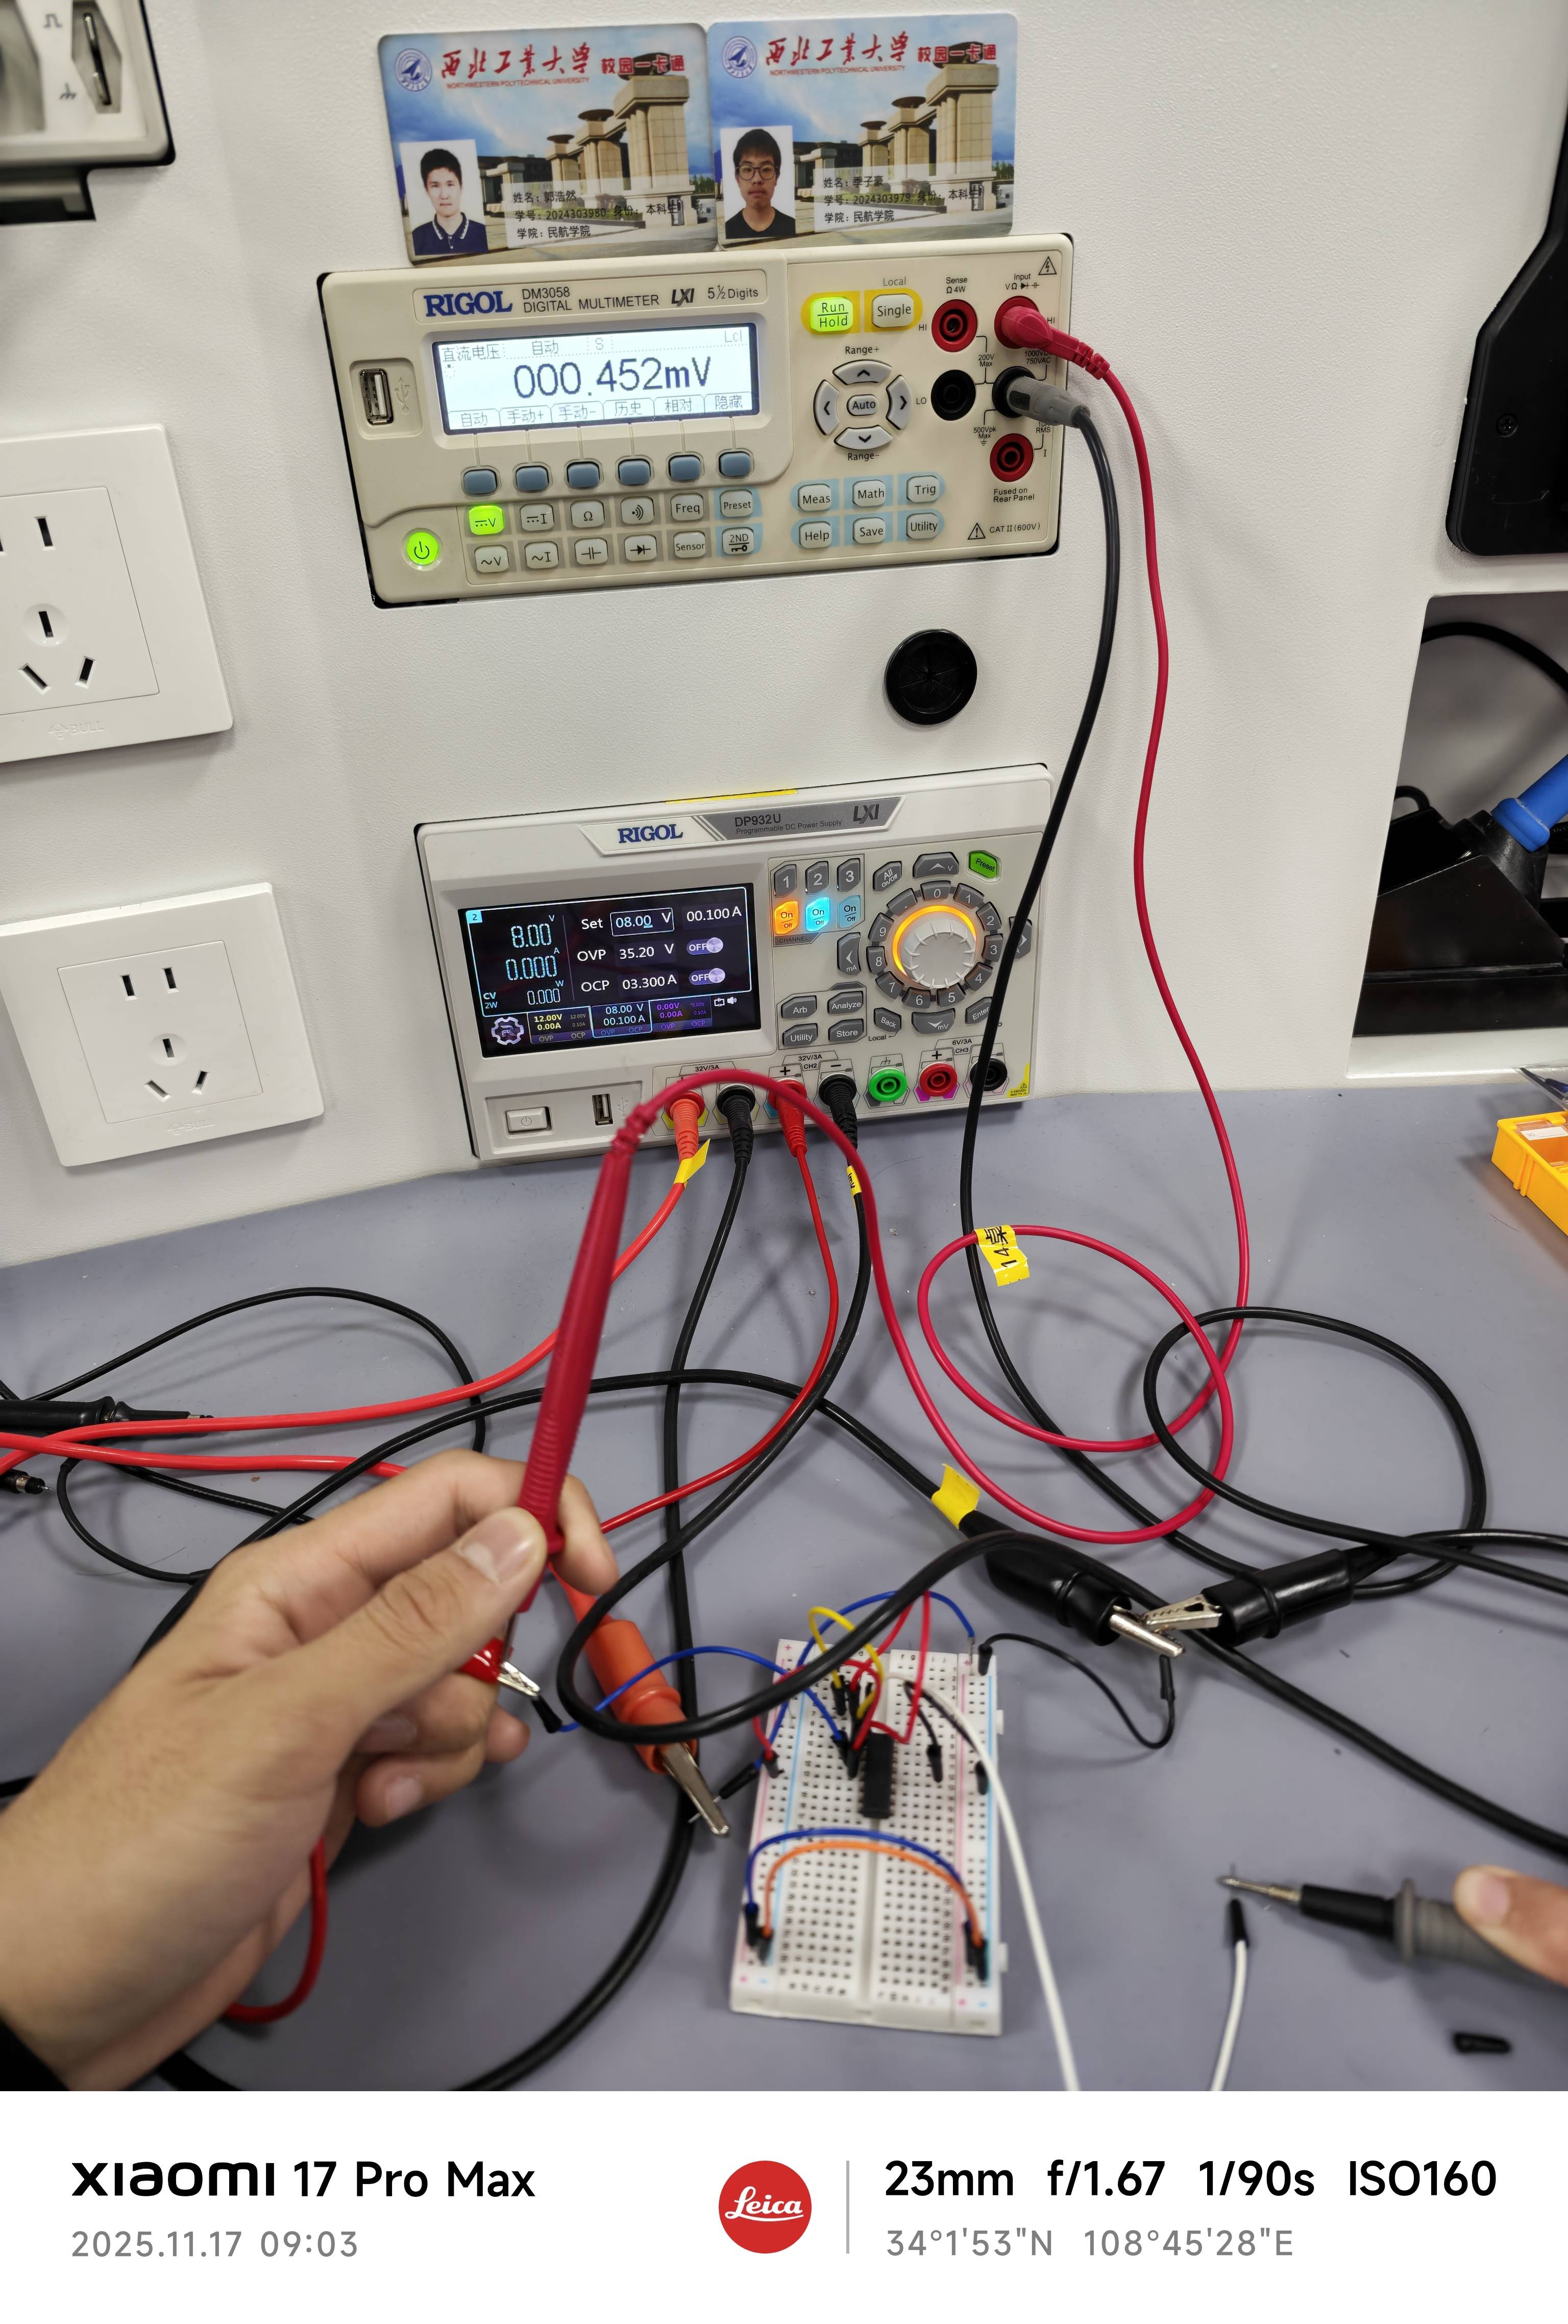
\includegraphics[width=\textwidth]{2_Op_amp/lm324_vos_photo.jpg} % <-- 替换为您的LM324失调电压实测图
        \caption{LM324 失调电压测量}
        \label{fig:lm324_vos}
    \end{subfigure}
    \hfill
    \begin{subfigure}[b]{0.48\textwidth}
        \centering
        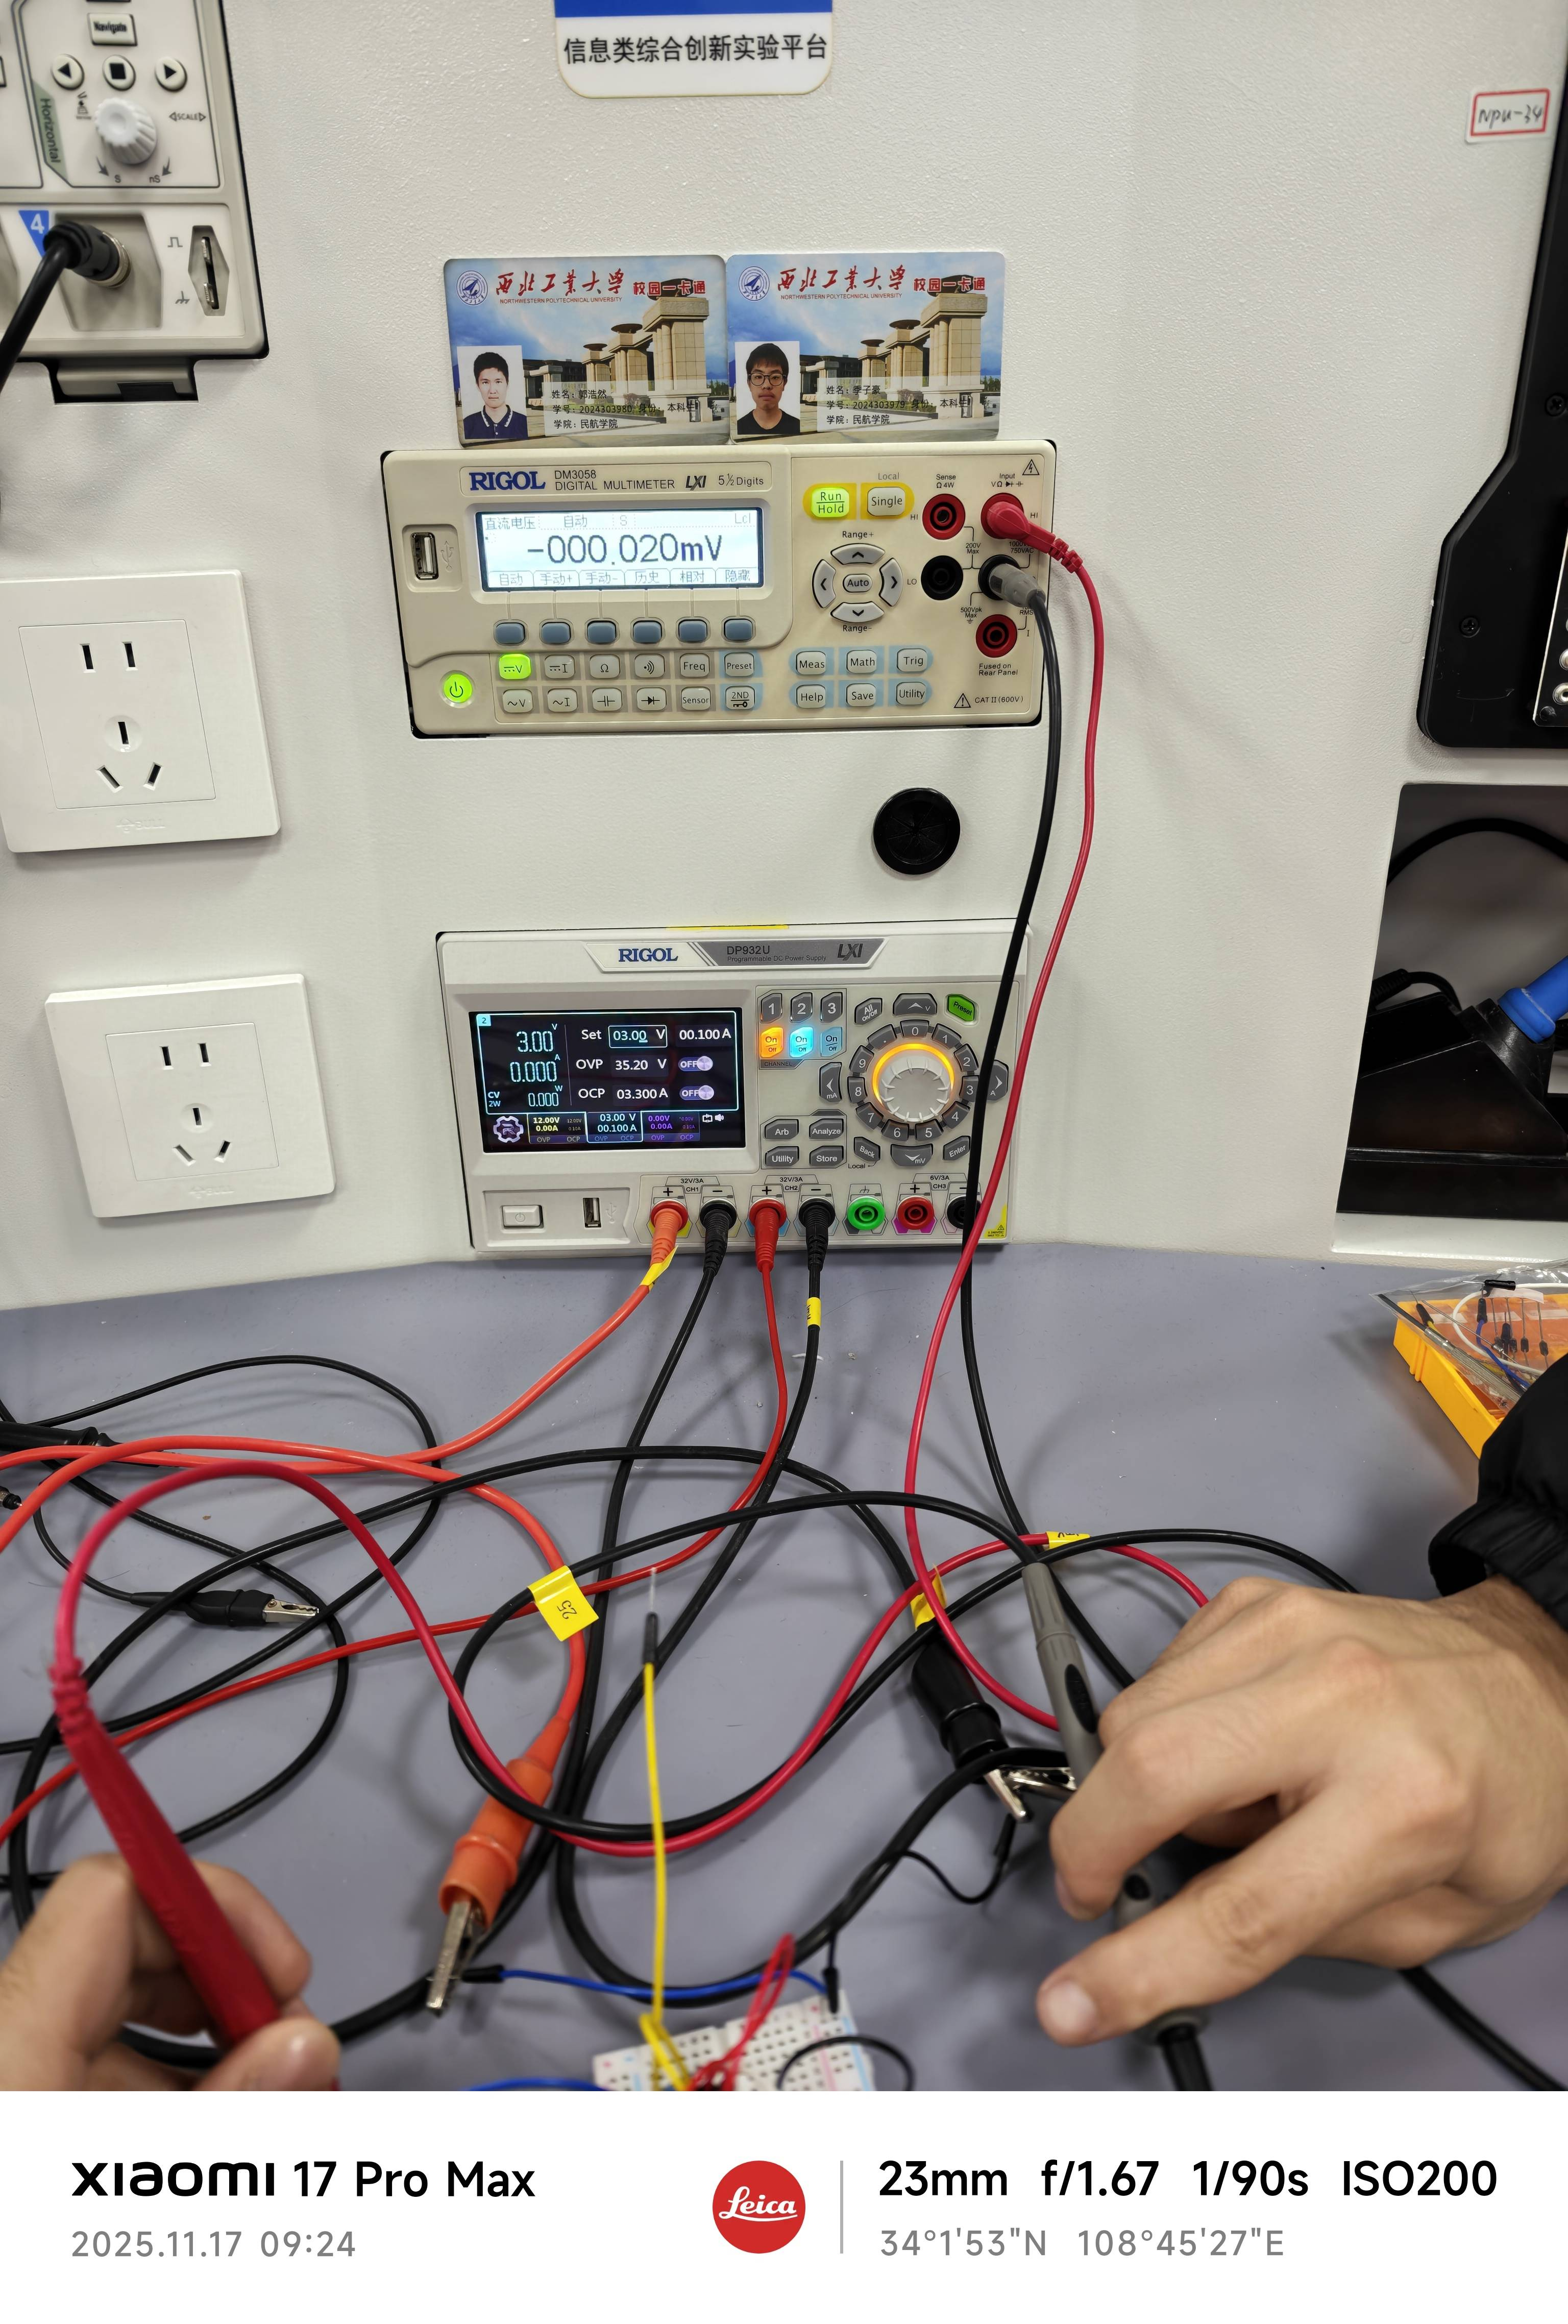
\includegraphics[width=\textwidth]{2_Op_amp/op07_vos_photo.jpg} % <-- 替换为您的OP07失调电压实测图
        \caption{OP07 失调电压测量}
        \label{fig:op07_vos}
    \end{subfigure}
    \caption{运放失调电压实测对比 (包含学号姓名纸条)}
    \label{fig:vos_measurement}
\end{figure}

根据万用表读数，记录结果如下：
\begin{itemize}
    \item LM324 运放失调电压: $V_{\text{OS, LM324}} = \SI{0.452}{\milli\volt}$
    \item OP07 运放失调电压: $V_{\text{OS, OP07}} = \SI{20}{\micro\volt}$
\end{itemize}
实验结果表明，高精度运放 OP07 的失调电压远小于通用型运放 LM324。

\subsubsection{共模输入范围测量}
在 \SI{12}{\volt} 单电源供电下，缓慢增加 LM324 电压跟随器的输入直流电压 $V_{\text{in}}$，并监测输出电压 $V_{\text{out}}$。当 $V_{\text{out}}$ 不再跟随 $V_{\text{in}}$ 时，即达到共模输入电压的上限。临界点的测量情况如图 \ref{fig:cmrr_measurement} 所示。

\begin{figure}[H]
    \centering
    \begin{subfigure}[b]{0.48\textwidth}
        \centering
        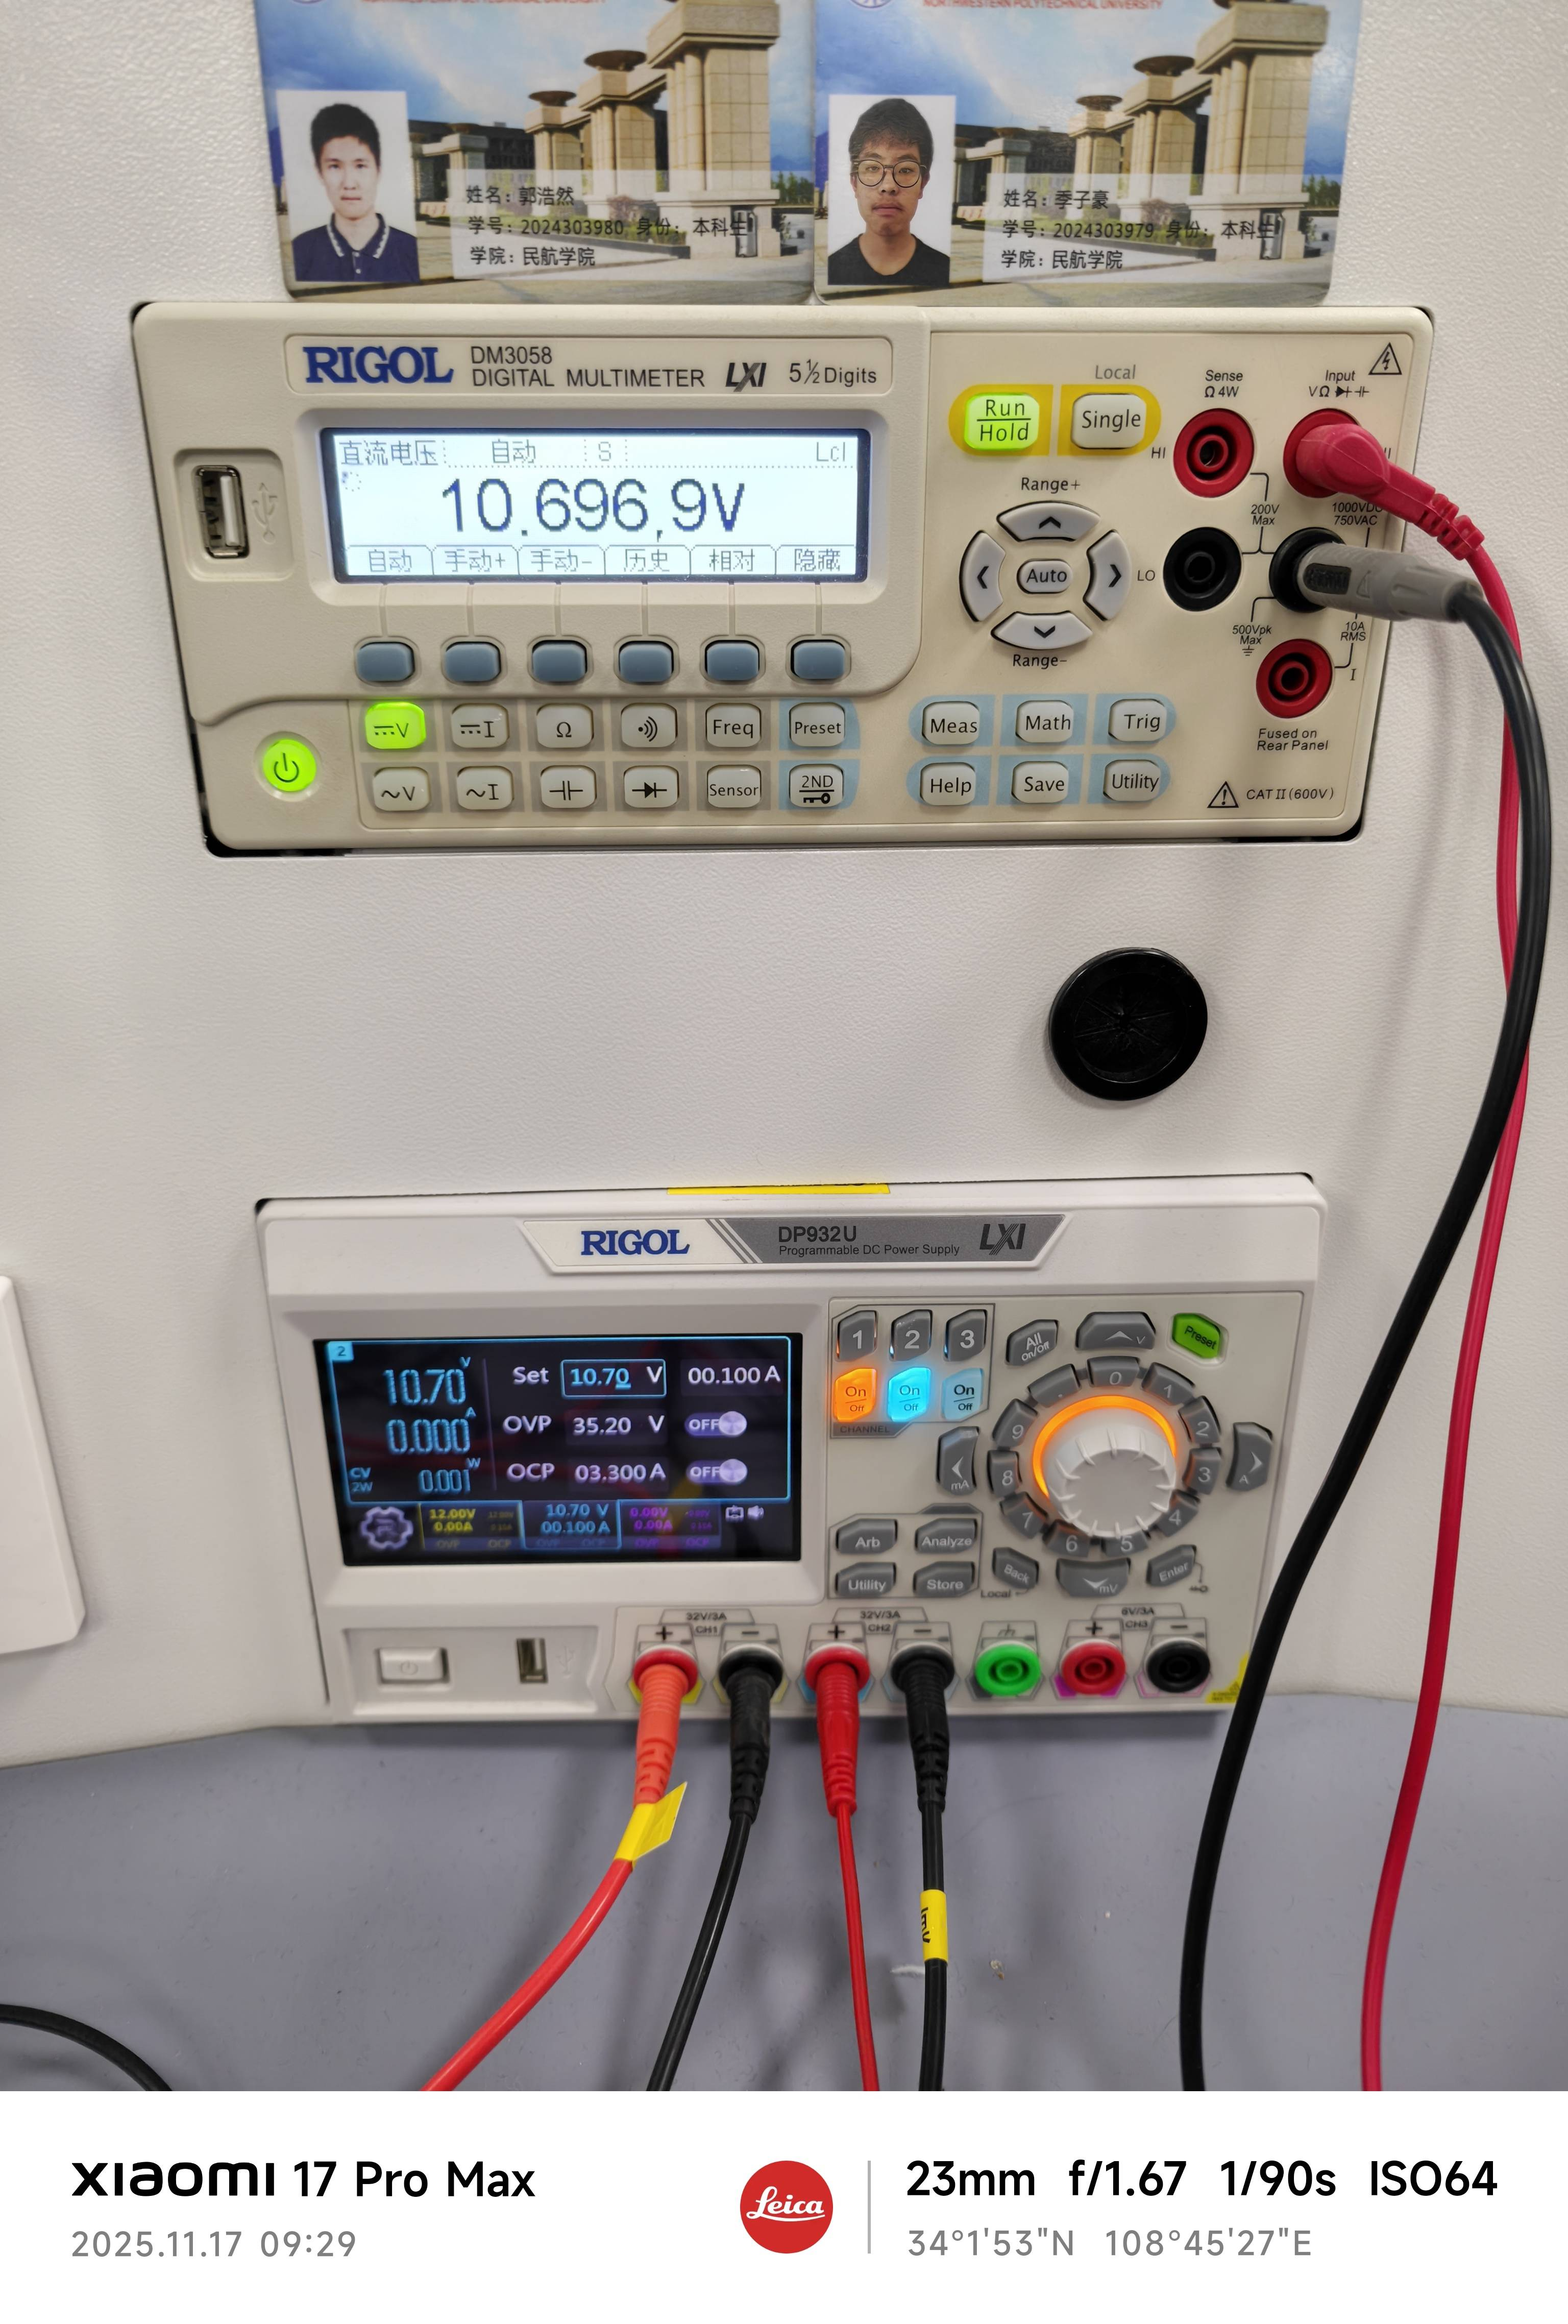
\includegraphics[width=\textwidth]{2_Op_amp/cmrr_follow.jpg} % <-- 替换为您的电压跟随正常时的实测图
        \caption{临界电压跟随状态 ($V_{\text{in}} = \SI{10.70}{\volt}$)}
        \label{fig:cmrr_follow}
    \end{subfigure}
    \hfill
    \begin{subfigure}[b]{0.48\textwidth}
        \centering
        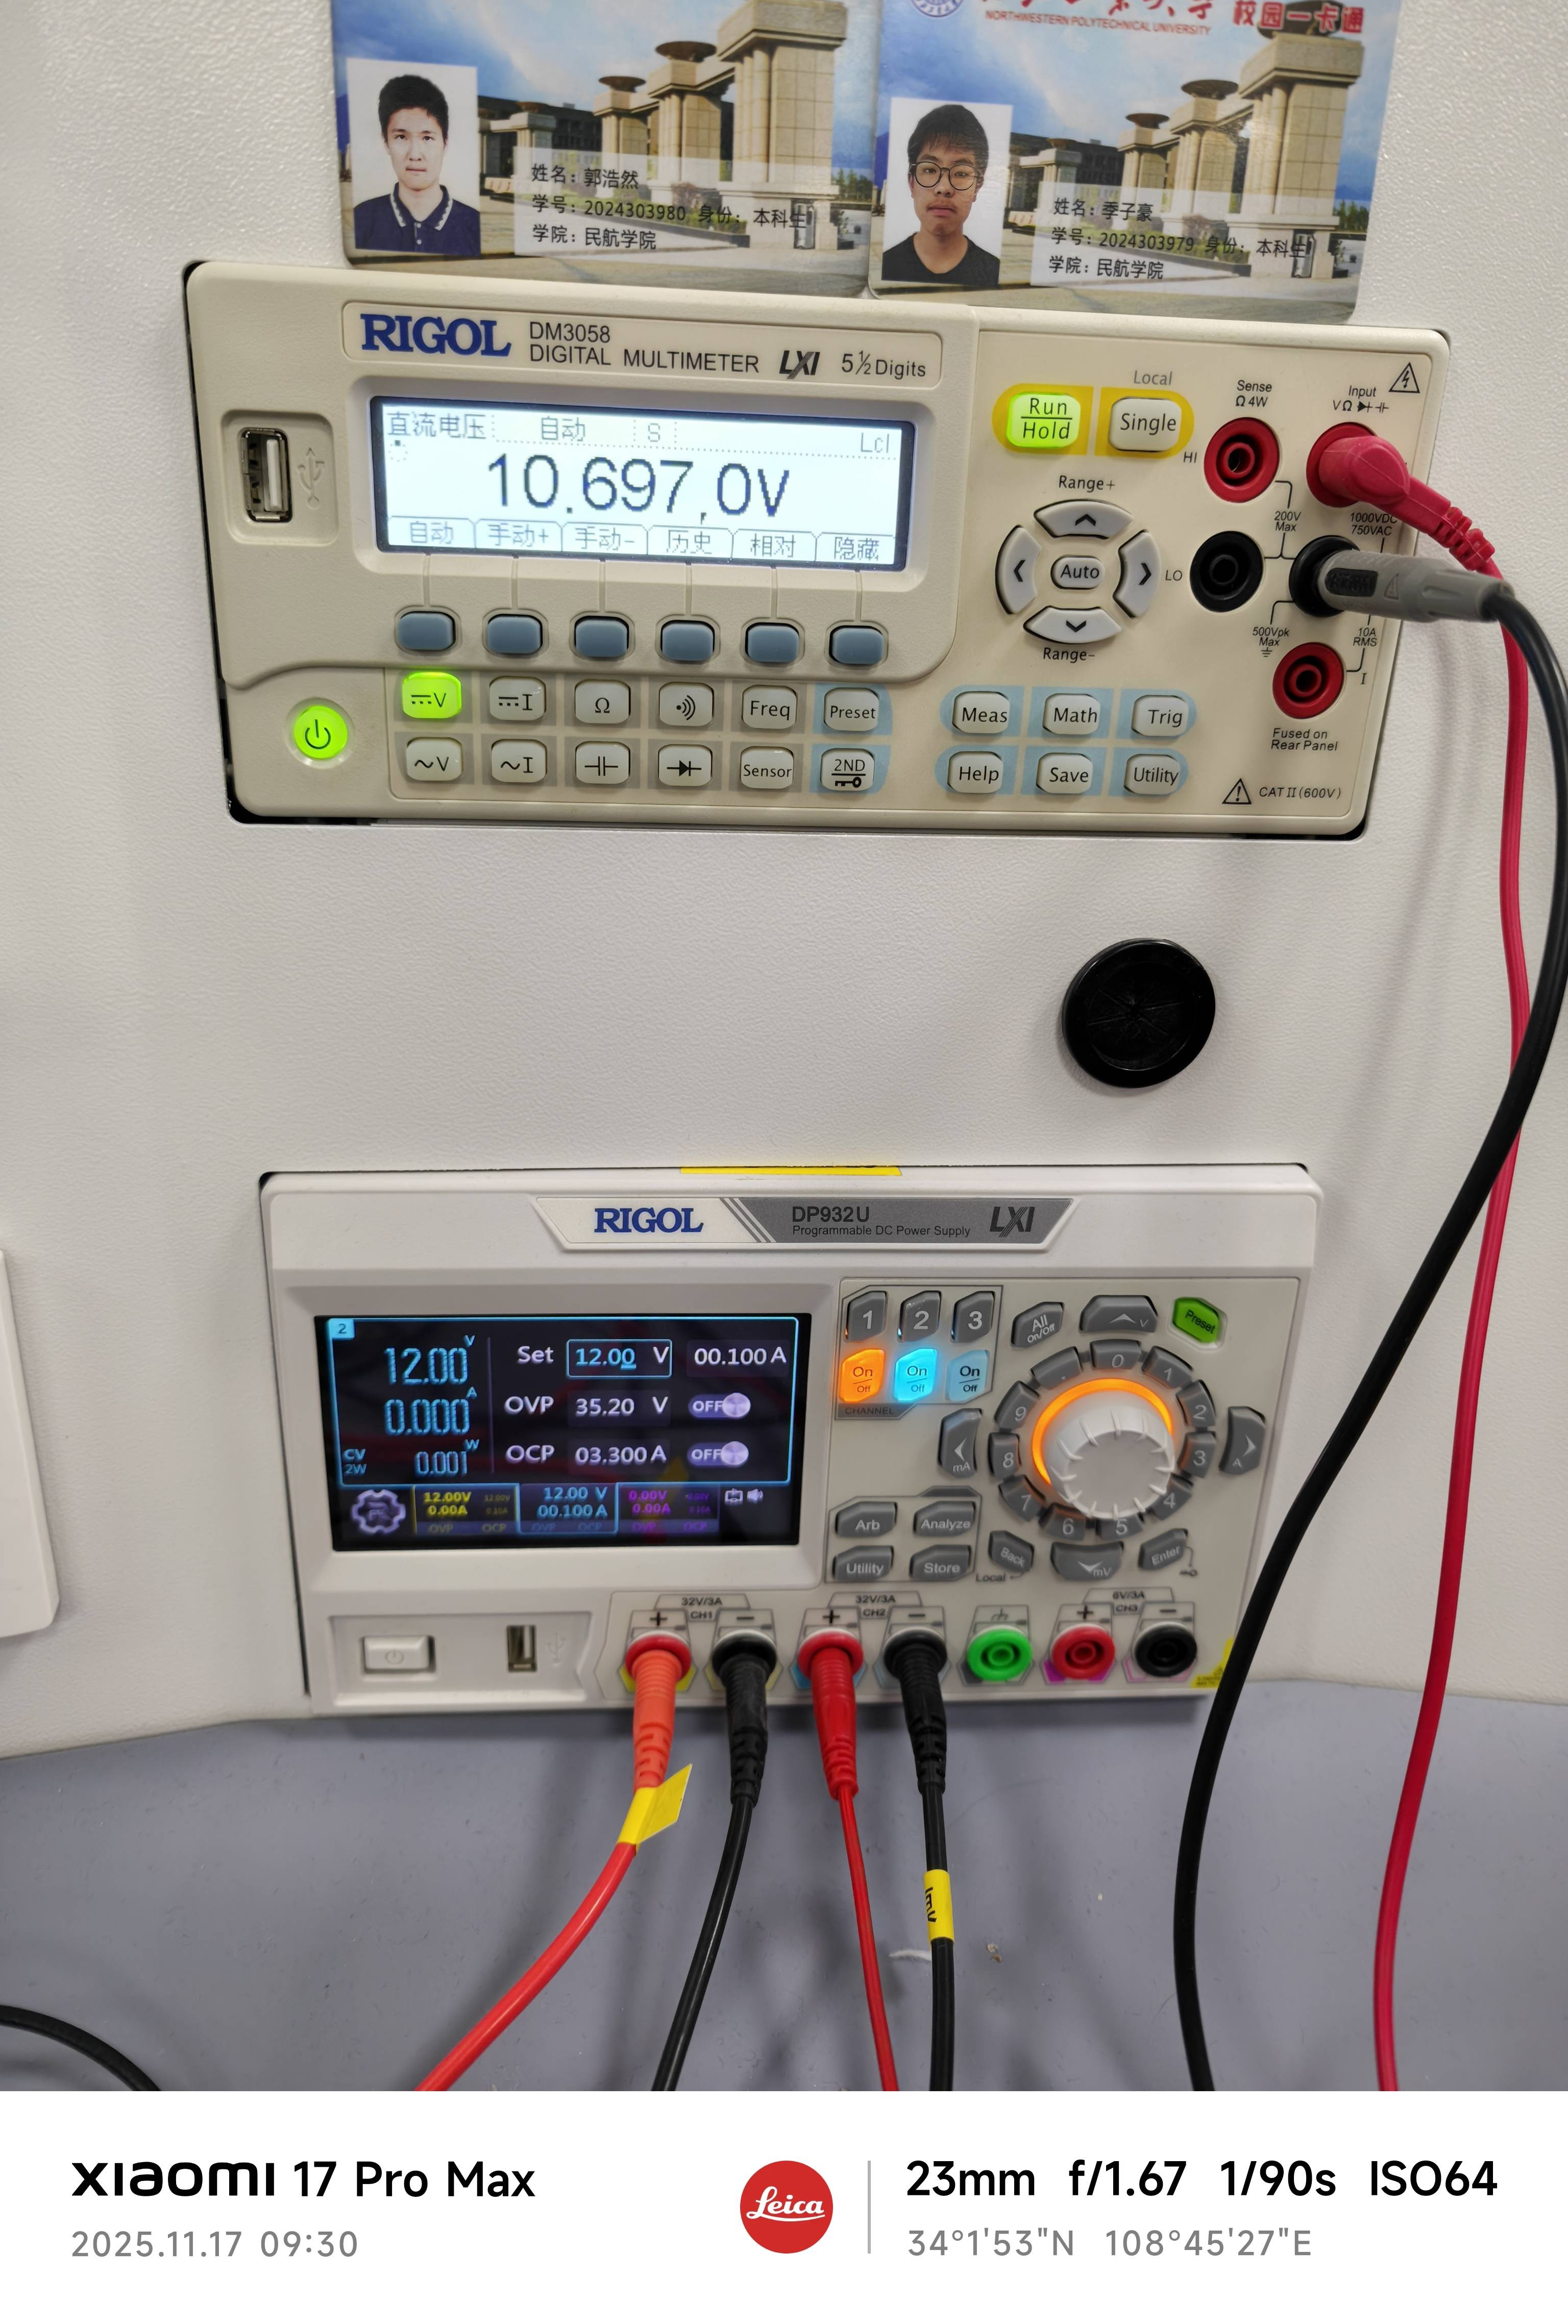
\includegraphics[width=\textwidth]{2_Op_amp/cmrr_limit.jpg} % <-- 替换为您的电压跟随失效时的实测图
        \caption{超出共模输入范围 ($V_{\text{in}} = \SI{12}{\volt}$)}
        \label{fig:cmrr_limit}
    \end{subfigure}
    \caption{共模输入范围临界点测试}
    \label{fig:cmrr_measurement}
\end{figure}

由实验数据可知：
\begin{itemize}
    \item 当 $V_{\text{in}} \le \SI{10.70}{\volt}$ 时, $V_{\text{out}} \approx V_{\text{in}}$，电路处于正常的电压跟随状态。
    \item 当 $V_{\text{in}}$ 增大至 $\SI{10.70}{\volt}$ 以上时, $V_{\text{out}}$ 保持在 \SI{10.697}{\volt} 不再上升，电压跟随状态消失。
\end{itemize}
因此，在 \SI{12}{\volt} 供电条件下，LM324 的共模输入范围的上限为 \SI{10.70}{\volt}，即共模输入范围为 $[\SI{0}{\volt}, \SI{10.70}{\volt}]$。

\subsubsection{幅频特性测试}
使用 LM324 构成的电压缓冲器，输入为叠加了直流偏置的正弦信号。通过改变频率，测量输出信号幅值的变化。中频、低频和高频（截止频率）下的示波器截图如图 \ref{fig:freq_response2} 所示。

\begin{figure}[H]
    \centering
    \begin{subfigure}[b]{0.48\textwidth}
        \centering
        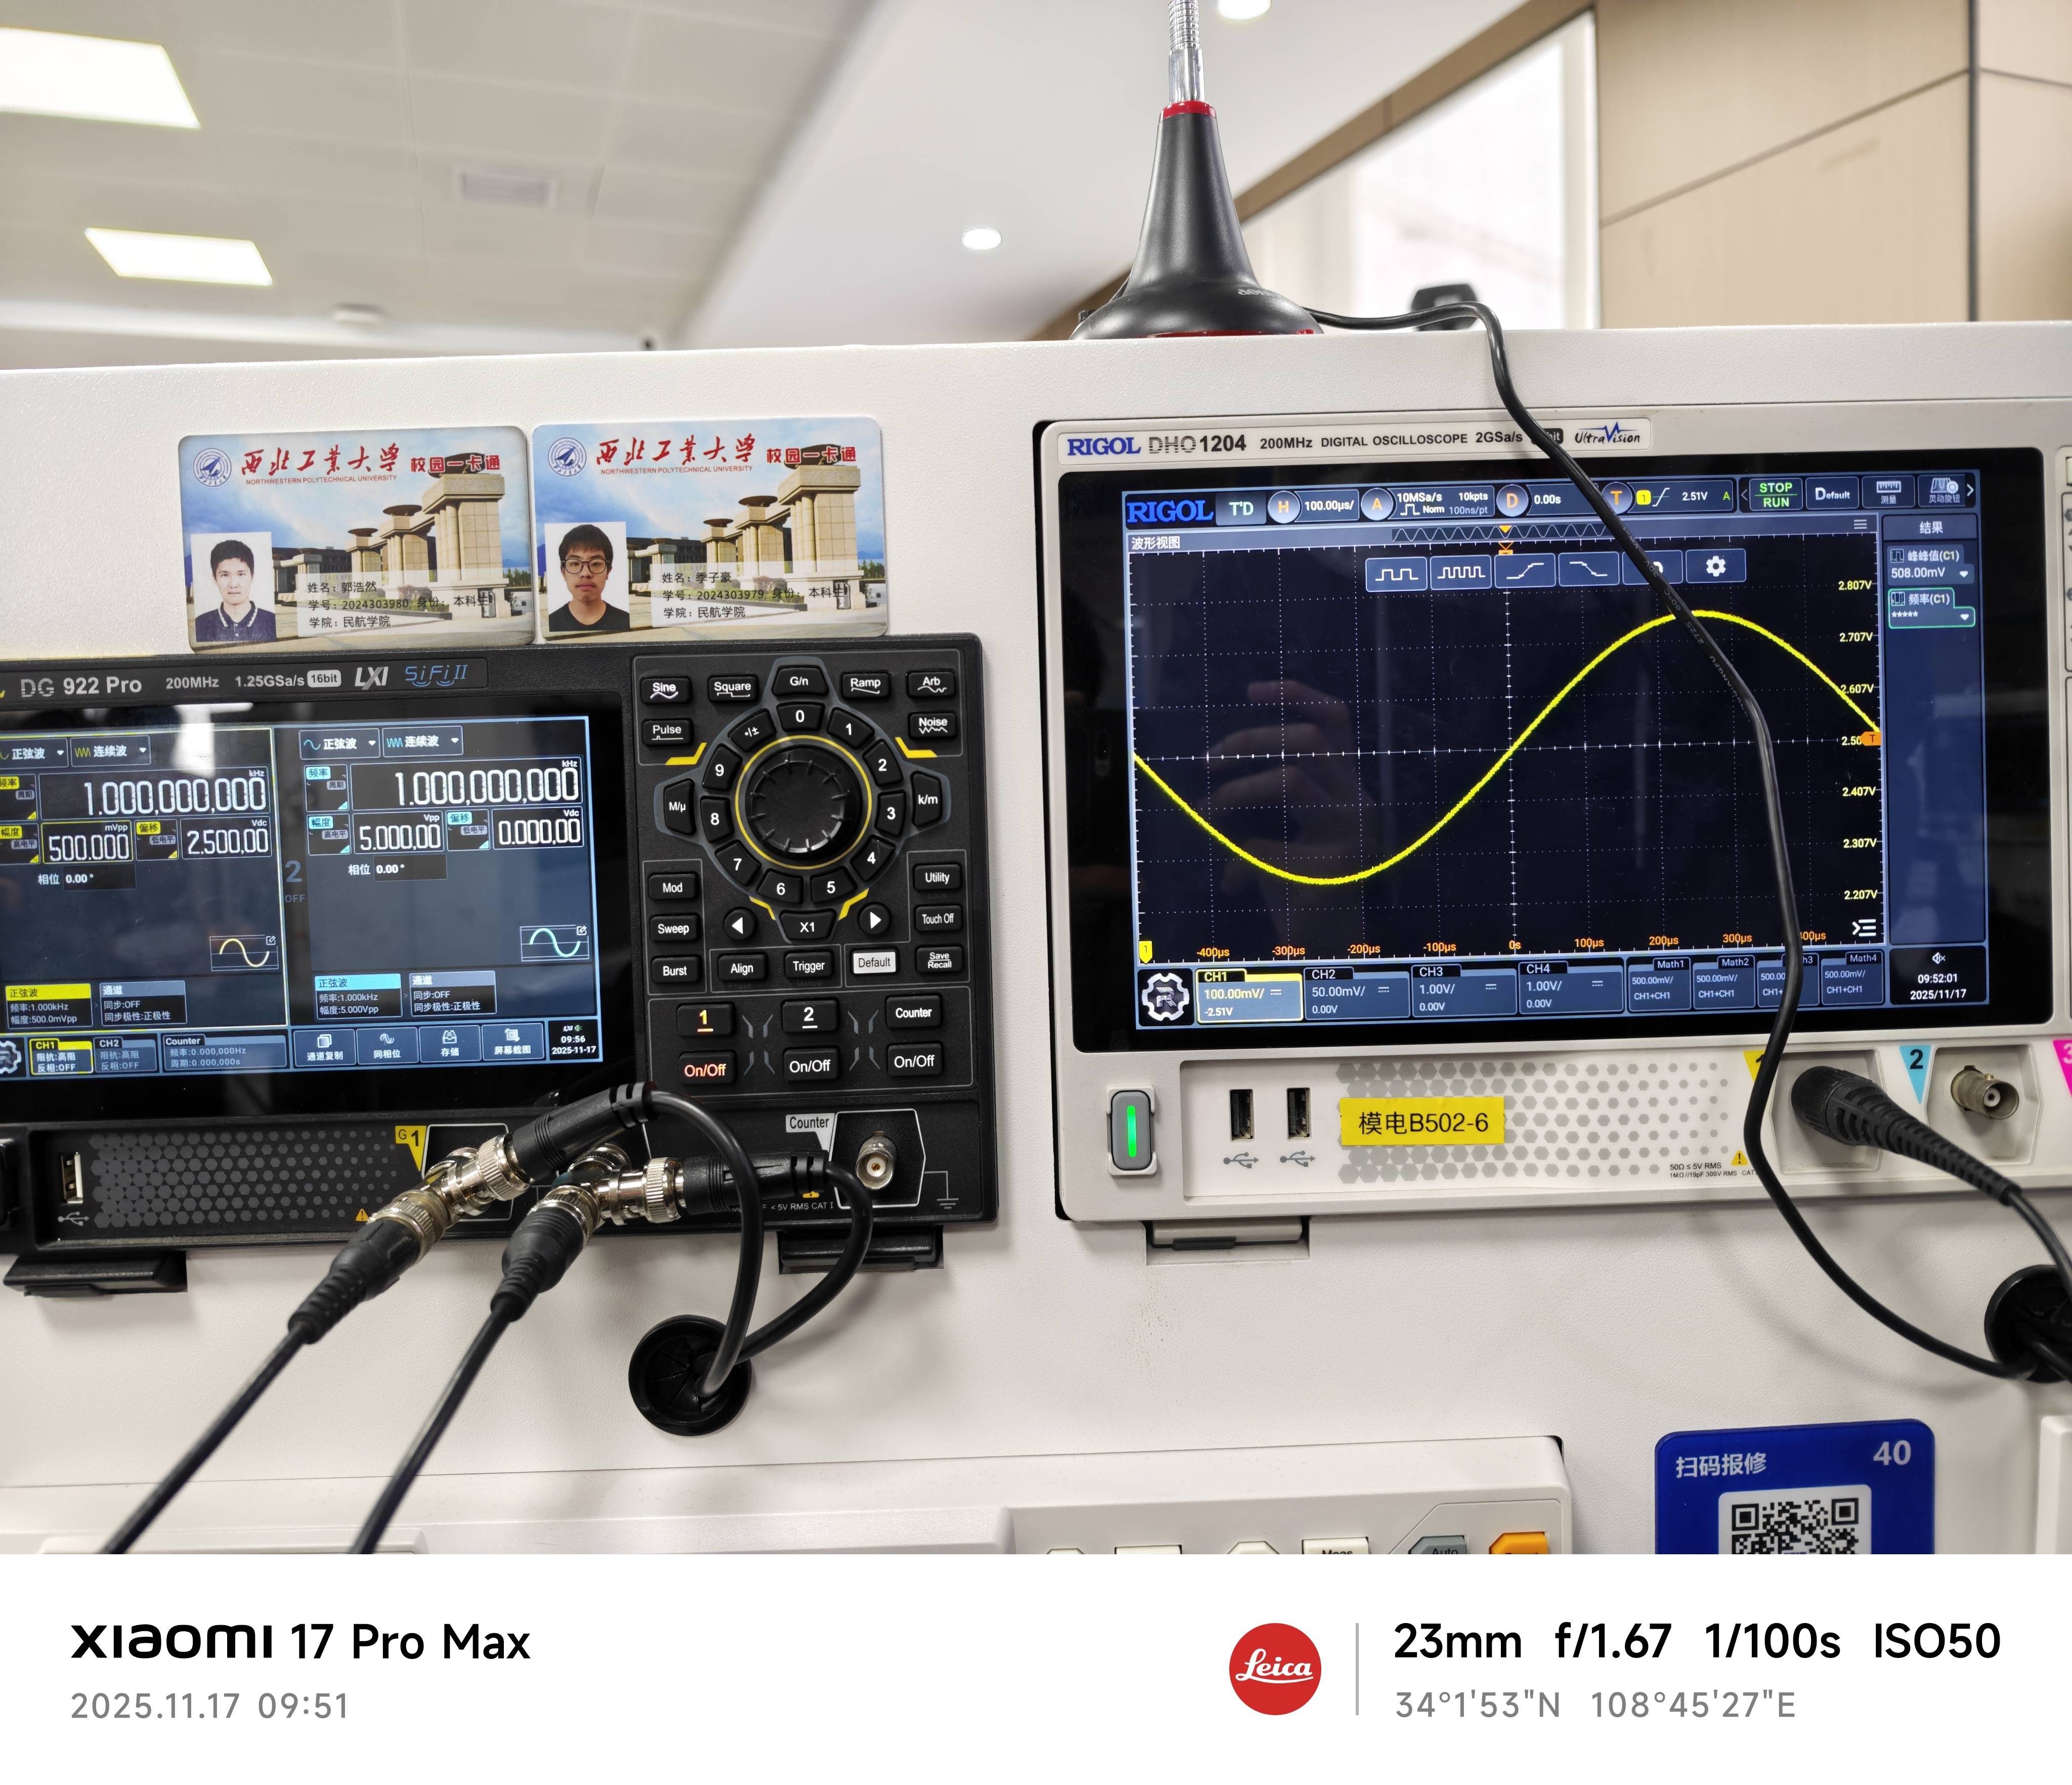
\includegraphics[width=\textwidth]{2_Op_amp/freq_mid.jpg} % <-- 替换为您的中频段响应实测图
        \caption{中频段 (\SI{1}{\kilo\hertz}) 响应}
        \label{fig:freq_mid}
    \end{subfigure}
    \hfill
    \begin{subfigure}[b]{0.48\textwidth}
        \centering
        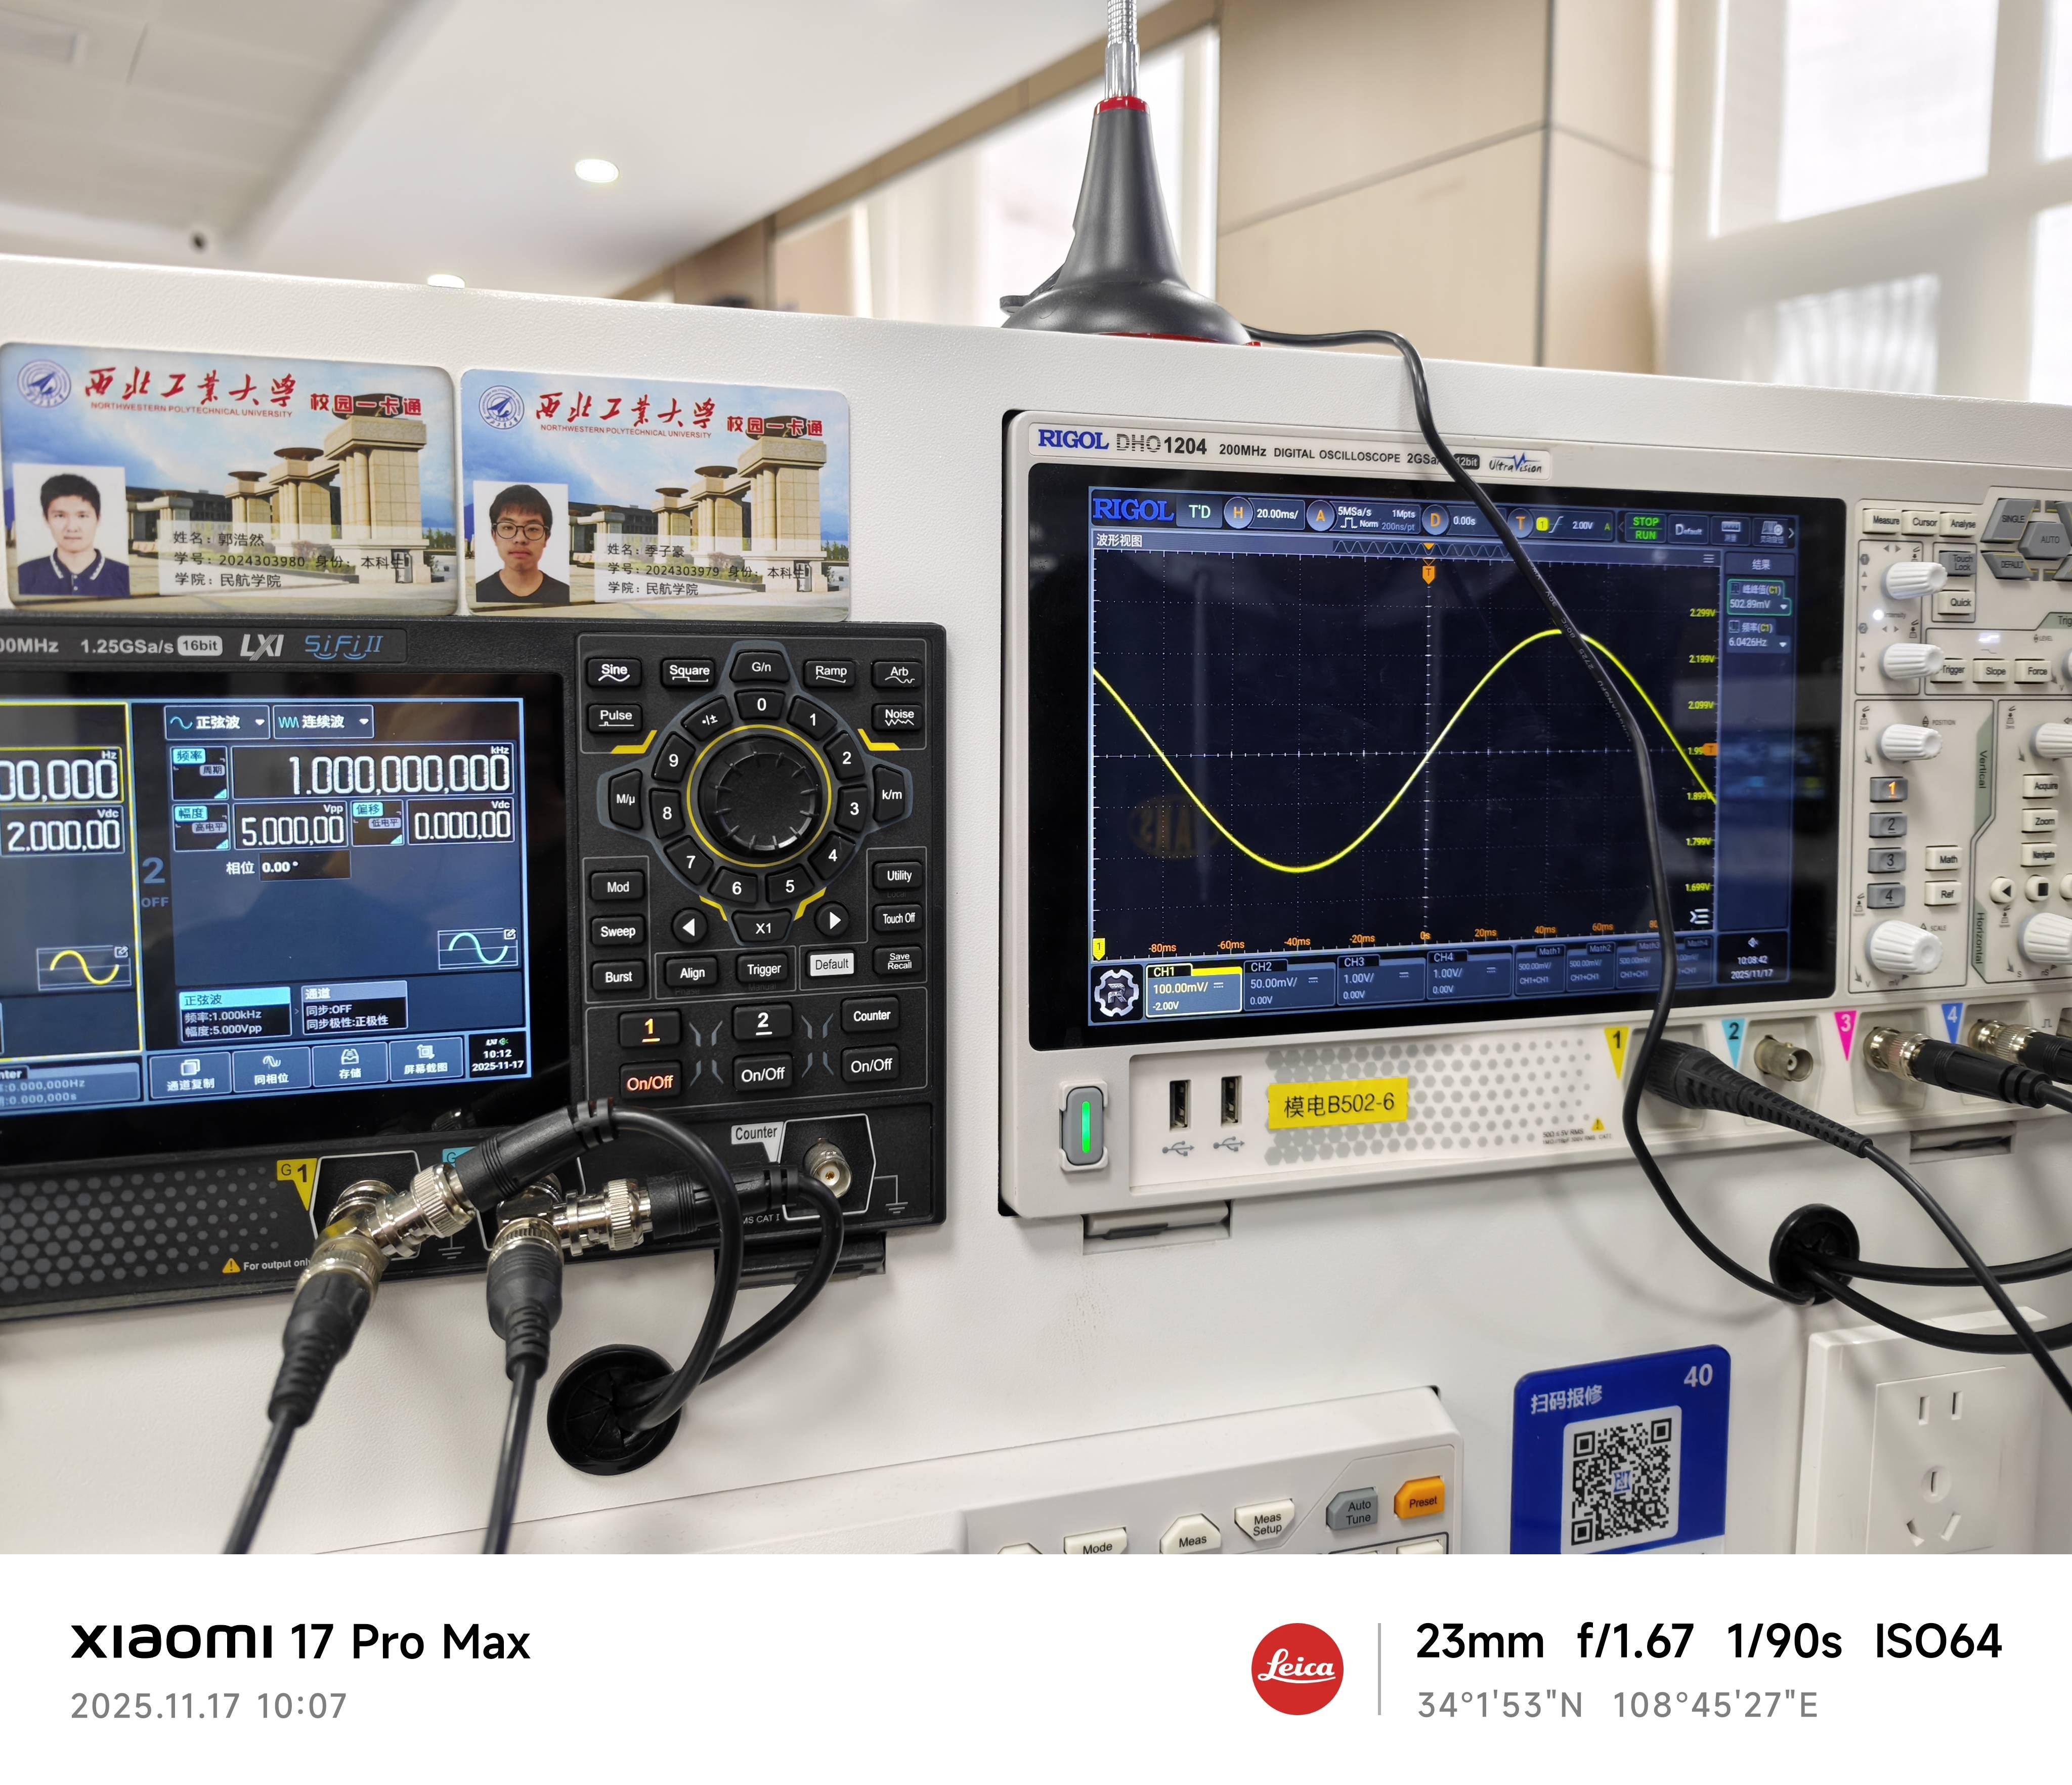
\includegraphics[width=\textwidth]{2_Op_amp/freq_low.jpg} % <-- 替换为您的低频段响应实测图
        \caption{低频段 (\SI{6}{\hertz}) 响应}
        \label{fig:freq_low}
    \end{subfigure}
    
    \vspace{1em} % 增加一点垂直间距
    
    \begin{subfigure}[b]{0.48\textwidth}
        \centering
        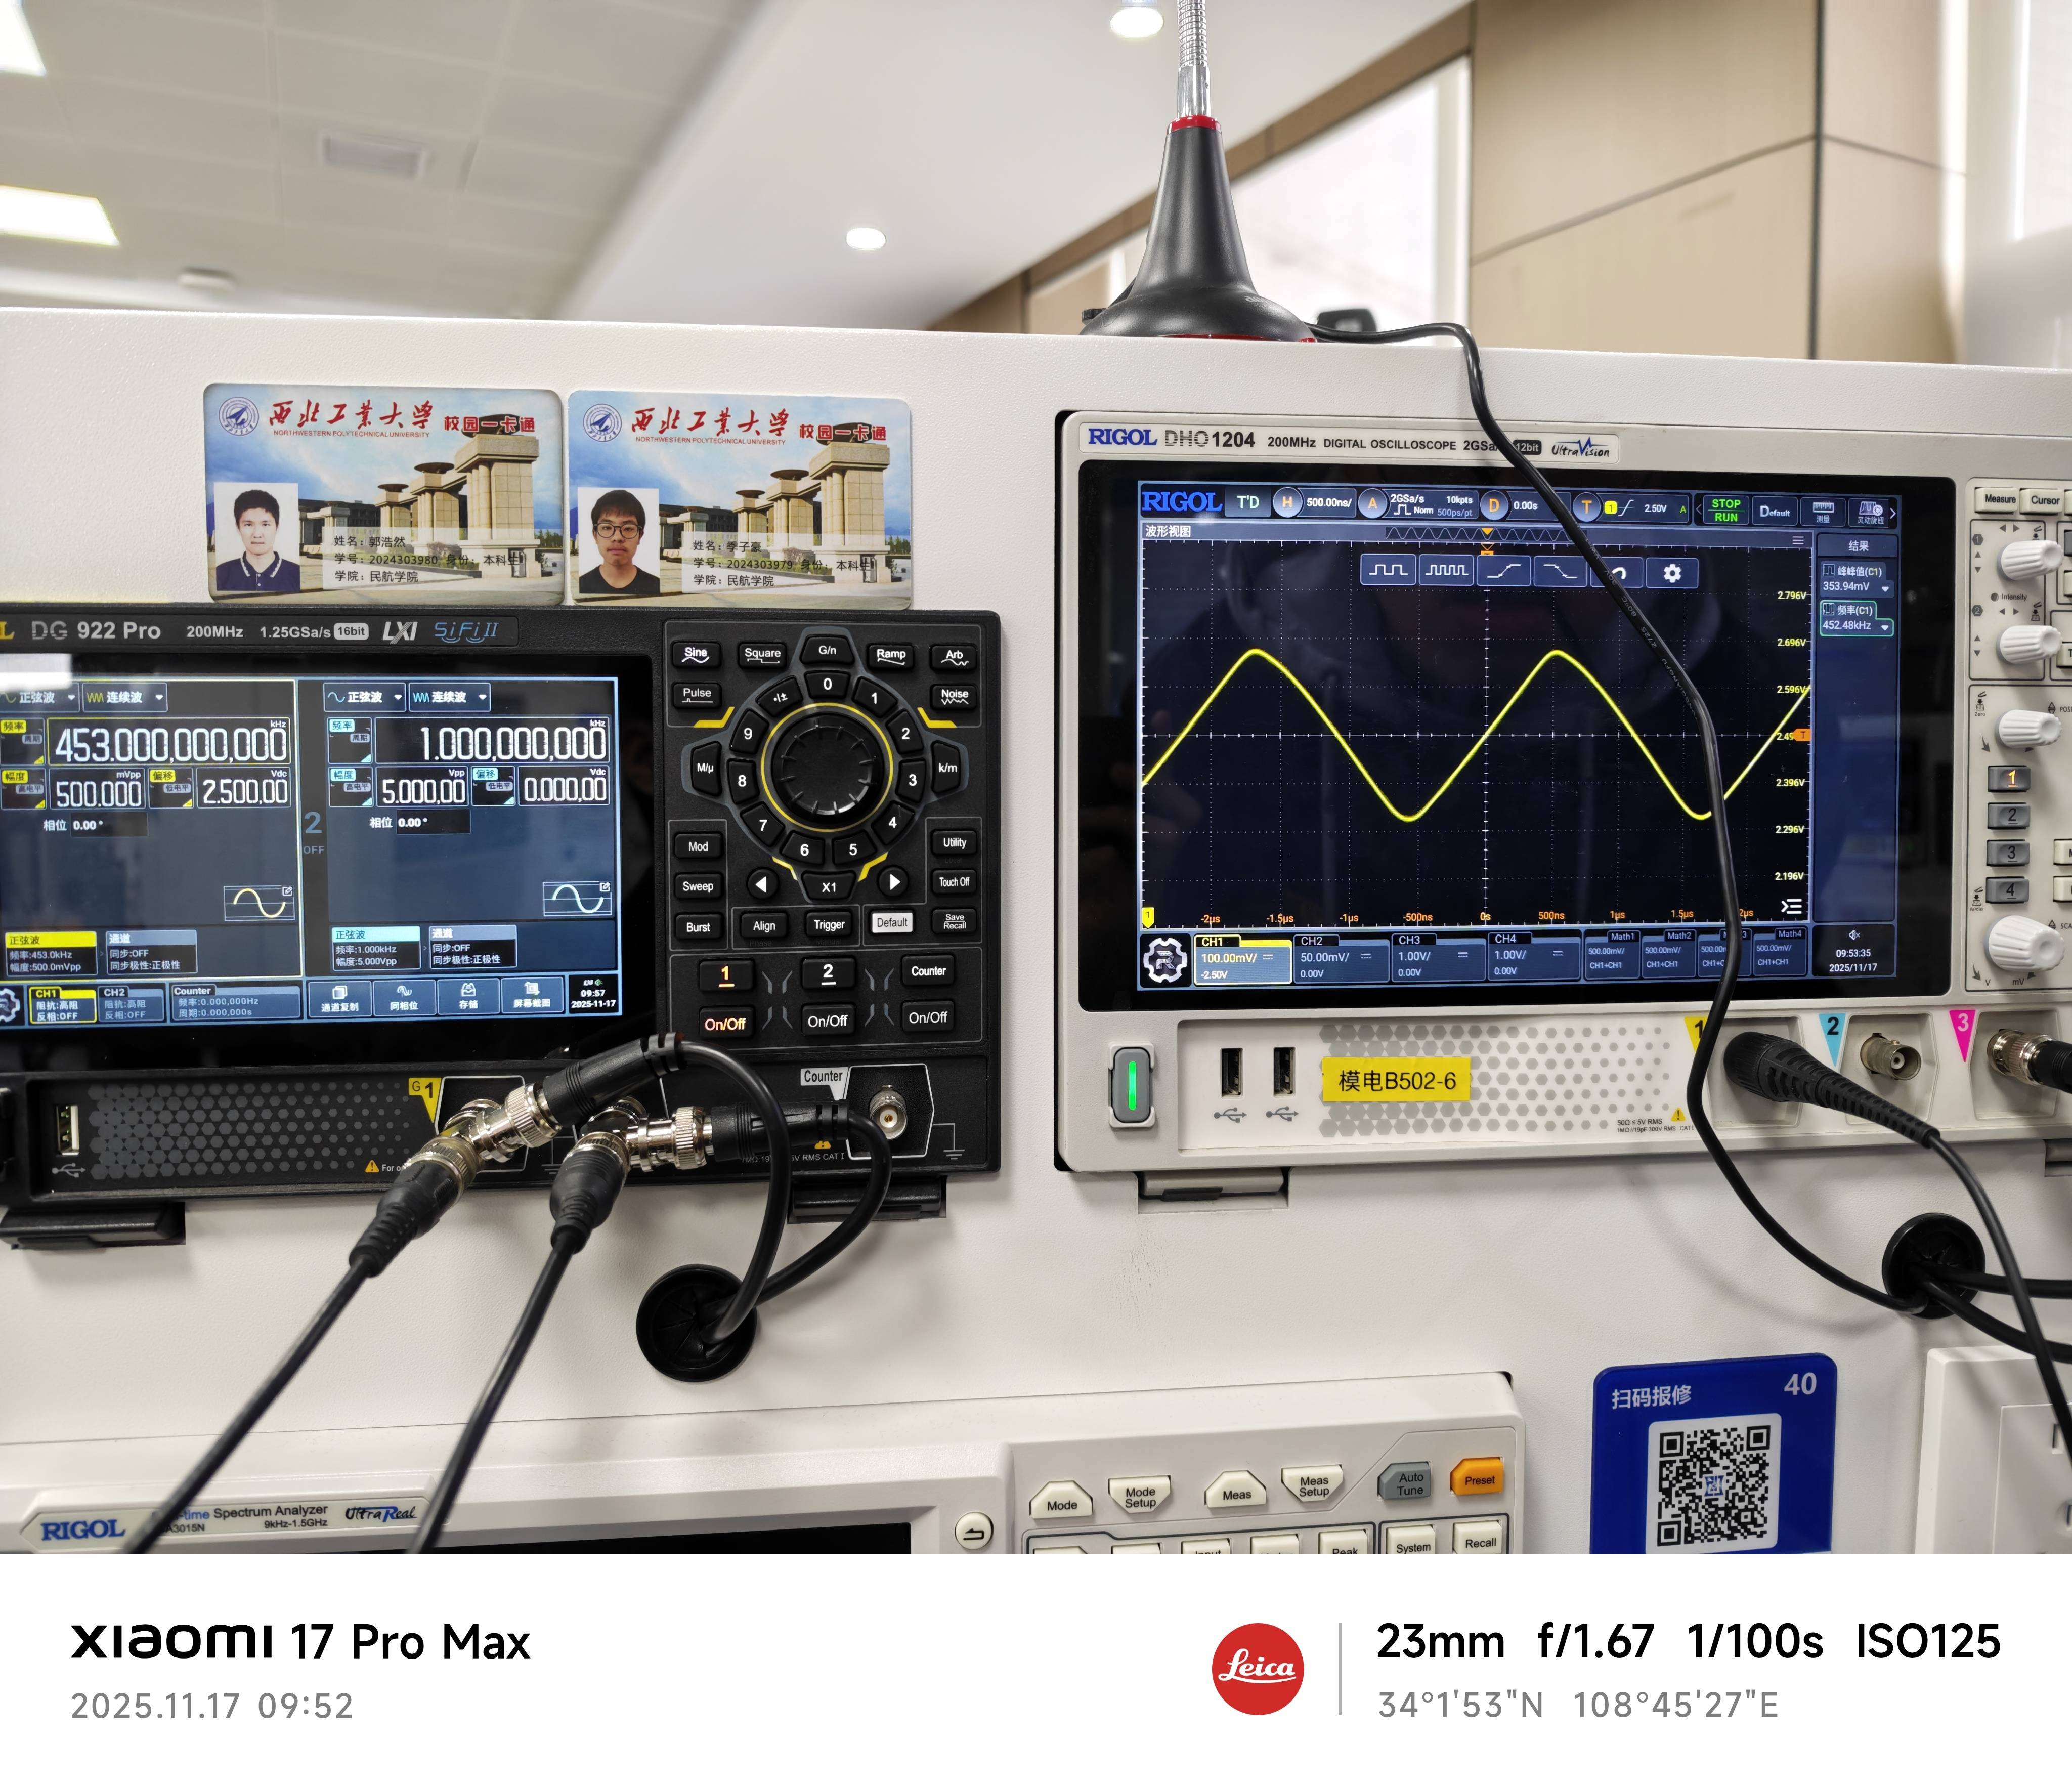
\includegraphics[width=\textwidth]{2_Op_amp/freq_high.jpg} % <-- 替换为您的高频段响应实测图
        \caption{上限截止频率 (\SI{453}{\kilo\hertz}) 响应}
        \label{fig:freq_high}
    \end{subfigure}
    \caption{LM324 电压缓冲器幅频特性测试}
    \label{fig:freq_response2}
\end{figure}

数据记录与计算过程如下：
\begin{enumerate}
    \item \textbf{中频增益测量：} 在中频段 (\SI{1}{\kilo\hertz})，测得输出电压幅值 $A_m = \SI{508.00}{\milli\volt}$。
    \item \textbf{-3dB 点计算：} 计算-3dB点对应的幅值：
    \[ A_{\text{-3dB}} = \frac{A_m}{\sqrt{2}} \approx 0.707 \times \SI{508.00}{\milli\volt} \approx \SI{358.46}{\milli\volt} \]
    \item \textbf{下限截止频率 $f_L$：} 降低频率至 \SI{1}{\hertz}，输出幅值无明显下降，仍为约 \SI{508}{\milli\volt}。因此，可认为下限截止频率 $f_L \approx \SI{0}{\hertz}$。
    \item \textbf{上限截止频率 $f_H$：} 提高频率，当频率达到 \SI{453}{\kilo\hertz} 时，测得输出幅值约为 \SI{358.46}{\milli\volt}，此值接近计算出的 \SI{358.46}{\milli\volt}。因此，可确定上限截止频率 $f_H \approx \SI{453}{\kilo\hertz}$。
    \item \textbf{通频带计算：}
    \[ f_{BW} = f_H - f_L \approx \SI{453}{\kilo\hertz} - \SI{0}{\hertz} = \SI{453}{\kilo\hertz} \]
\end{enumerate}

% ===================================================================
% 章节：结论与分析
% ===================================================================
\section{结论与分析}\label{sec:opamp_conclusion}
\begin{enumerate}
    \item \textbf{数据结论：} 本次实验成功测量了 LM324 和 OP07 两种运放的关键指标。
    \begin{itemize}
        \item \textbf{失调电压：} 测得 LM324 的 $V_{\text{OS}} = \SI{0.452}{\milli\volt}$，OP07 的 $V_{\text{OS}} = \SI{20}{\micro\volt}$。结果直观地体现了高精度运放 (OP07) 在直流特性上的巨大优势。
        \item \textbf{共模范围：} LM324 在 \SI{12}{\volt} 单电源供电下的共模输入范围为 $[\SI{0}{\volt}, \SI{10.70}{\volt}]$，与规格书中的理论值 $V_{CC} - \SI{1.5}{\volt} = \SI{10.5}{\volt}$ 高度吻合。
        \item \textbf{幅频特性：} LM324 构成的电压缓冲器下限截止频率接近直流，上限截止频率约为 \SI{453}{\kilo\hertz}，通频带为 \SI{453}{\kilo\hertz}。
    \end{itemize}
    
    \item \textbf{误差分析：} 实验中主要的误差来源在于测量上限截止频率 $f_H$ 的过程。由于需要手动调节信号发生器的频率并同时观察示波器上的电压读数，很难精确地使输出幅值恰好为 $A_m/\sqrt{2}$。在临界点附近，频率的微小变化可能导致幅值的较大跳动，且示波器读数本身也存在误差。为减小此误差，应在临界点附近进行更精细的频率微调，并进行多次测量取平均值。
    
    \item \textbf{实验总结：} 通过本次实验，我们不仅验证了芯片规格书中的关键参数，还通过实际操作加深了对输入失调电压、共模输入范围和幅频特性等核心概念的理解。实验结果符合理论预期，证明了实验方案的有效性。
\end{enumerate}




\end{document}
